%%%%%%%%%%%%%%%%%%%%%%%%%%%%%%%%%%%%%%%%%
% Beamer Presentation
% LaTeX Template
% Version 1.0 (10/11/12)
%
% This template has been downloaded from:
% http://www.LaTeXTemplates.com
%
% License:
% CC BY-NC-SA 3.0 (http://creativecommons.org/licenses/by-nc-sa/3.0/)
%
%%%%%%%%%%%%%%%%%%%%%%%%%%%%%%%%%%%%%%%%%

%----------------------------------------------------------------------------------------
%	PACKAGES AND THEMES
%----------------------------------------------------------------------------------------

\documentclass[unknownkeysallowed]{beamer}

\mode<presentation> {

% The Beamer class comes with a number of default slide themes
% which change the colors and layouts of slides. Below this is a list
% of all the themes, uncomment each in turn to see what they look like.

% \usetheme{default}
%\usetheme{AnnArbor}
%\usetheme{Antibes}
%\usetheme{Bergen}
%\usetheme{Berkeley}
%\usetheme{Berlin}
%\usetheme{Boadilla}
%\usetheme{CambridgeUS}
%\usetheme{Copenhagen}
%\usetheme{Darmstadt}
%\usetheme{Dresden}
%\usetheme{Frankfurt}
%\usetheme{Goettingen}
%\usetheme{Hannover}
%\usetheme{Ilmenau}
%\usetheme{JuanLesPins}
% \usetheme{Luebeck}
\usetheme{Madrid}
%\usetheme{Malmoe}
% \usetheme{Marburg}
%\usetheme{Montpellier}
%\usetheme{PaloAlto}
%\usetheme{Pittsburgh}
%\usetheme{Rochester}
%\usetheme{Singapore}
%\usetheme{Szeged}
%\usetheme{Warsaw}

% As well as themes, the Beamer class has a number of color themes
% for any slide theme. Uncomment each of these in turn to see how it
% changes the colors of your current slide theme.

%\usecolortheme{albatross}
%\usecolortheme{beaver}
%\usecolortheme{beetle}
%\usecolortheme{crane}
%\usecolortheme{dolphin}
%\usecolortheme{dove}
%\usecolortheme{fly}
%\usecolortheme{lily}
%\usecolortheme{orchid}
%\usecolortheme{rose}
%\usecolortheme{seagull}
%\usecolortheme{seahorse}
%\usecolortheme{whale}
%\usecolortheme{wolverine}

%\setbeamertemplate{footline} % To remove the footer line in all slides uncomment this line
%\setbeamertemplate{footline}[page number] % To replace the footer line in all slides with a simple slide count uncomment this line

%\setbeamertemplate{navigation symbols}{} % To remove the navigation symbols from the bottom of all slides uncomment this line
}

\usepackage{graphicx, url} % Allows including images
\usepackage{booktabs} % Allows the use of \toprule, \midrule and \bottomrule in tables
\usepackage[caption=false,font=footnotesize]{subfig}

\usepackage{cite}
\usepackage{amsmath,amssymb,amsfonts, comment, xcolor}
% \usepackage{algorithmic}
% \usepackage{textcomp}
\usepackage{xcolor}
\usepackage{multirow}
% \usepackage{caption}
\usepackage{balance}
% \usepackage{array}
% \usepackage[final]{graphicx}
% \usepackage{subcaption}
% \usepackage{pgfplots}
% \usepackage{pgfplotstable}
% \usepackage{sfmath}
% \usepackage{lipsum}
\usepackage{graphicx}

\setbeamertemplate{caption}[numbered]

% usecolortheme{beaver}
\usepackage{textpos}

% Change color
\definecolor{UBCblue}{rgb}{0.04706, 0.13725, 0.26667}
\definecolor{USFgreen}{rgb}{0.14, 0.545, 0.14} % 0.13, 0.545, 0.13} 0.1, 0.35, 0.1
\definecolor{USFgreen2}{RGB}{0,103,71}
\usecolortheme[named=USFgreen2]{structure}

%----------------------------------------------------------------------------------------
%	TITLE PAGE
%----------------------------------------------------------------------------------------

\title[Signal Synthesis for Affects Detection]{Synthesizing Physiological and Motion Data for Stress and Meditation Detection} % The short title appears at the bottom of every slide, the full title is only on the title page

% \subtitle{Facial Dynamics Learning} 

\author[Taufeeq and Canavan]{Md Taufeeq Uddin, Shaun Canavan} % Your name
\institute[USF] % Your institution as it will appear on the bottom of every slide, may be shorthand to save space
{
Computer Vision \& Pattern Recognition - Affective Vision Lab \newline 
University of South Florida, FL, USA \\ 
\includegraphics[height=2cm,width=2cm]{figs/USF_logo_v2.jpg} \\ % Your institution for the title page
\medskip
\texttt{mdtaufeeq@mail.usf.edu, scanavan@usf.edu} % Your email address
}
\date[AAAC ACII2019: ML4AD]{AAAC ACII 2019: ML4AD Workshop, Cambridge, UK} % Date, can be changed to a custom date

\begin{document}

\begin{frame}
\titlepage % Print the title page as the first slide
\end{frame}

% \addtobeamertemplate{frametitle}{}{%
% \begin{textblock*}{100mm}(.95\textwidth,-1cm)
% 
\includegraphics[height=1cm,width=1cm]{figs/USF_logo_5.jpg}
% \end{textblock*}}


\begin{frame}
\frametitle{Overview} % Table of contents slide, comment this block out to remove it
\tableofcontents % Throughout your presentation, if you choose to use \section{} and \subsection{} commands, these will automatically be printed on this slide as an overview of your presentation
\end{frame}

%----------------------------------------------------------------------------------------
%	PRESENTATION SLIDES
%----------------------------------------------------------------------------------------


%------------------------------------------------
\section{Motivation}
%------------------------------------------------

\begin{frame}
\frametitle{Motivation}

\textit{Improving mental health via synthesizing signal for predicting affective states } \newline 

\begin{enumerate}[1.]
    \pause \item Can we synthesize (predict) physiological and motion signal (data) ahead of time?
    \pause \item If so, can we use the data to predict affective states?
\end{enumerate}


\end{frame}


%------------------------------------------------
\section{Contribution}
%------------------------------------------------

\begin{frame}
\frametitle{Contributions}

\begin{enumerate}[-]
    \item Synthesized (predicted) physiological signal ahead of time
    
    \item Predicted affective states from the synthetic data
    
    \item Published first baseline results on meditation (/ relaxed state) detection from WESAD dataset.
\end{enumerate}

\end{frame}


%------------------------------------------------
\section{Model: Physiological and Motion Data Synthesis}
%------------------------------------------------

\begin{frame}
\frametitle{Physiological and Motion Data Synthesis}

\begin{figure}
  \centering
  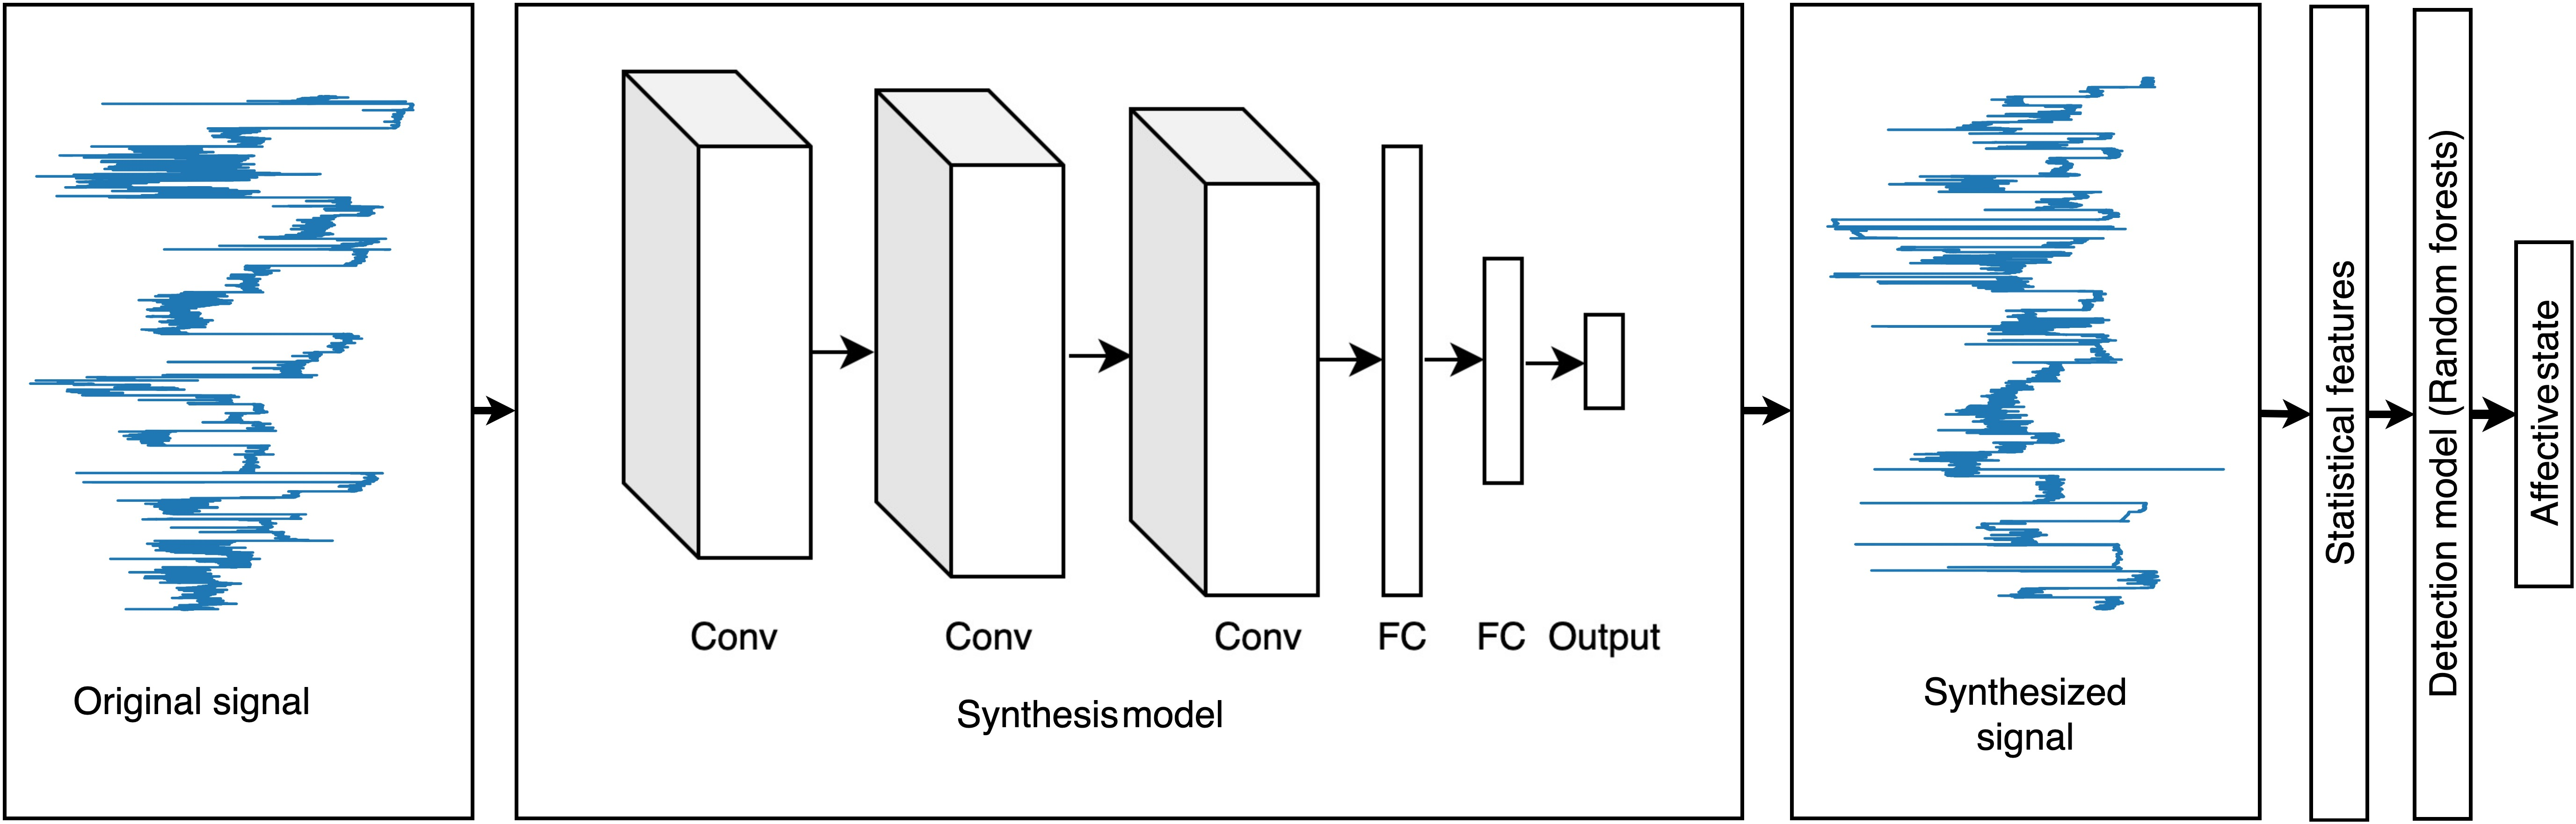
\includegraphics[width=.85\textwidth]{figs/syn_framework.jpg}
  \label{fig:overview}
\end{figure}

\begin{enumerate}[Step 1.]
    \pause \item Predict (synthesize) futuristic data from current and previous observations
    \pause \item Feed features (computed from the synthetic data) to affect detection model
\end{enumerate}

\end{frame}





%------------------------------------------------
\section{Data}
%------------------------------------------------

\begin{frame}
\frametitle{WESAD (Schmidt et al., ICMI 2018) Dataset}

\begin{enumerate}[-]
    \item Devices: RespiBAN and Empatica E4
    \item Signals: Acceleration, ECG, EMG, EDA, Temperature, Respiration 
    \item Subjects: 15 (12 males and 3 females) grad students
    \item Data Collection
    \begin{enumerate}[1.]
        \item \textbf{Neutral}: induce neutral affective state. ~20 mins long
        \item \textbf{Amusement}: induce happy state. ~6.5 mins long
        \item \textbf{Stress}: induce stress via public speaking and mental math tasks.  ~10 mins long
        \item \textbf{Meditation (/ relaxed)}: breathing exercise. ~7 mins long
    \end{enumerate}
    
\end{enumerate}

\textbf{Note}: \textit{In this work, we only used data collected via RespiBAN device}

\end{frame}


%------------------------------------------------
\section{Experiments and Analysis}
%------------------------------------------------

\begin{frame}
\frametitle{Experiments}

\begin{enumerate}[-]
    \item \textbf{Data Preprocessing}
        \begin{enumerate}[1.]
            \item Smooth raw signal via Savitz-Golay filter
            \item Normalized the data in between [0, 1] \newline 
        \end{enumerate}
        
    \pause \item \textbf{Convolutional neural network (CNN)} for synthesis \newline
    
    \item \textbf{Random forest} for affective states classification \newline 
    
    \pause \item \textbf{Model validation}: 3-fold subject independent (non-overlapping subjects) \newline 
\end{enumerate}

\end{frame}


\begin{frame}
\frametitle{Performance: Synthesis}

Input feature vector size = 25 \newline 
CCC Score: higher $\longrightarrow$ better

\textbf{Time T1}: Use \textbf{0.25} second of data to predict \textbf{0.01} second of data

\begin{table}
	\renewcommand{\arraystretch}{1.3}
	% \caption{Synthesis results on WESAD dataset using proposed 1DCNN.
	% }
	\label{syn_ccc_s_list}
	\centering
	\begin{tabular}{llll}
		\hline
		\bfseries Signal  & \bfseries  & \bfseries CCC score & \bfseries \\
		       &  Time T1 &  - & - \\
		\hline
		ACC X &   0.9909$\pm$0.0054 \\ % & 0.9856$\pm$0.0119 & 0.9899$\pm$0.0014 \\
		%\hline
		ACC Y &   0.9675$\pm$0.0272 \\ % & 0.9711$\pm$0.0081 & 0.7882$\pm$0.2552 \\
		%\hline
		ACC Z  &   0.9957$\pm$0.003 \\ % & 0.992$\pm$0.0026 & 0.9943$\pm$0.0024\\
		%\hline
		ECG &   0.8104$\pm$0.0327 \\ % & 0.5001$\pm$0.0922 & 0.3995$\pm$0.0602 \\
		%\hline
		EMG &   0.4381$\pm$0.6313 \\ % & 0.5837$\pm$0.0561 & 0.3407$\pm$0.4757 \\
		EDA &   0.9928$\pm$0.0012 \\ % & 0.9964$\pm$0.0009 & 0.9927$\pm$0.0036 \\    
		TEMP &  0.95$\pm$0.0268 \\ % & 0.9401$\pm$0.0437 & 0.7405$\pm$0.1785 \\
		RESP &  0.9895$\pm$0.0009 \\ % & 0.9697$\pm$0.0065 & 0.9563$\pm$0.0094\\
		\hline
	\end{tabular}
\end{table}

\end{frame}



\begin{frame}
\frametitle{Performance: Synthesis}

Input feature vector size = 25 \newline 
CCC Score: higher $\longrightarrow$ better

\textbf{Time T2}: Use \textbf{1} second of data to predict \textbf{0.04} second of data


\begin{table}
	\renewcommand{\arraystretch}{1.3}
	% \caption{Synthesis results on WESAD dataset using proposed 1DCNN.
	% }
	\label{syn_ccc_s_list}
	\centering
	\begin{tabular}{llll}
		\hline
		\bfseries Signal  & \bfseries  & \bfseries CCC score & \bfseries \\
		       &  Time T1 &  Time T2 & - \\
		\hline
		ACC X &   0.9909$\pm$0.0054 & 0.9856$\pm$0.0119 \\ % & 0.9899$\pm$0.0014 \\
		%\hline
		ACC Y &   0.9675$\pm$0.0272 & 0.9711$\pm$0.0081 \\ % & 0.7882$\pm$0.2552 \\
		%\hline
		ACC Z  &   0.9957$\pm$0.003 & 0.992$\pm$0.0026 \\ % & 0.9943$\pm$0.0024\\
		%\hline
		ECG &   0.8104$\pm$0.0327 & 0.5001$\pm$0.0922 \\ % & 0.3995$\pm$0.0602 \\
		%\hline
		EMG &   0.4381$\pm$0.6313 & 0.5837$\pm$0.0561 \\ % & 0.3407$\pm$0.4757 \\
		EDA &   0.9928$\pm$0.0012 & 0.9964$\pm$0.0009 \\ % & 0.9927$\pm$0.0036 \\    
		TEMP &  0.95$\pm$0.0268 & 0.9401$\pm$0.0437  \\ % & 0.7405$\pm$0.1785 \\
		RESP &  0.9895$\pm$0.0009 & 0.9697$\pm$0.0065 \\ % & 0.9563$\pm$0.0094\\
		\hline
	\end{tabular}
\end{table}

\end{frame}



\begin{frame}
\frametitle{Performance: Synthesis}

Input feature vector size = 25 \newline 
CCC Score: higher $\longrightarrow$ better

\textbf{Time T3}: Use \textbf{2} seconds of data to predict \textbf{0.1} second of data

\begin{table}
	\renewcommand{\arraystretch}{1.3}
	% \caption{Synthesis results on WESAD dataset using proposed 1DCNN.
	% }
	\label{syn_ccc_s_list}
	\centering
	\begin{tabular}{llll}
		\hline
		\bfseries Signal  & \bfseries & \bfseries CCC score & \bfseries \\
		       &  Time T1 &  Time T2 & Time T3 \\
		\hline
		ACC X &   0.9909$\pm$0.0054 & 0.9856$\pm$0.0119 & 0.9899$\pm$0.0014 \\
		%\hline
		ACC Y &   0.9675$\pm$0.0272 & 0.9711$\pm$0.0081 & 0.7882$\pm$0.2552 \\
		%\hline
		ACC Z  &   0.9957$\pm$0.003 & 0.992$\pm$0.0026 & 0.9943$\pm$0.0024\\
		%\hline
		ECG &   0.8104$\pm$0.0327 & 0.5001$\pm$0.0922 & 0.3995$\pm$0.0602 \\
		%\hline
		EMG &   0.4381$\pm$0.6313 & 0.5837$\pm$0.0561 & 0.3407$\pm$0.4757 \\
		EDA &   0.9928$\pm$0.0012 & 0.9964$\pm$0.0009 & 0.9927$\pm$0.0036 \\    
		TEMP &  0.95$\pm$0.0268 & 0.9401$\pm$0.0437 & 0.7405$\pm$0.1785 \\
		RESP &  0.9895$\pm$0.0009 & 0.9697$\pm$0.0065 & 0.9563$\pm$0.0094\\
		\hline
	\end{tabular}
\end{table}

\end{frame}



%------------------------------------------------

\begin{frame}
\frametitle{Sample Signals (Original and Synthesis)}

% \section{Experimental Design and Results}
\begin{figure}
  \centering
%   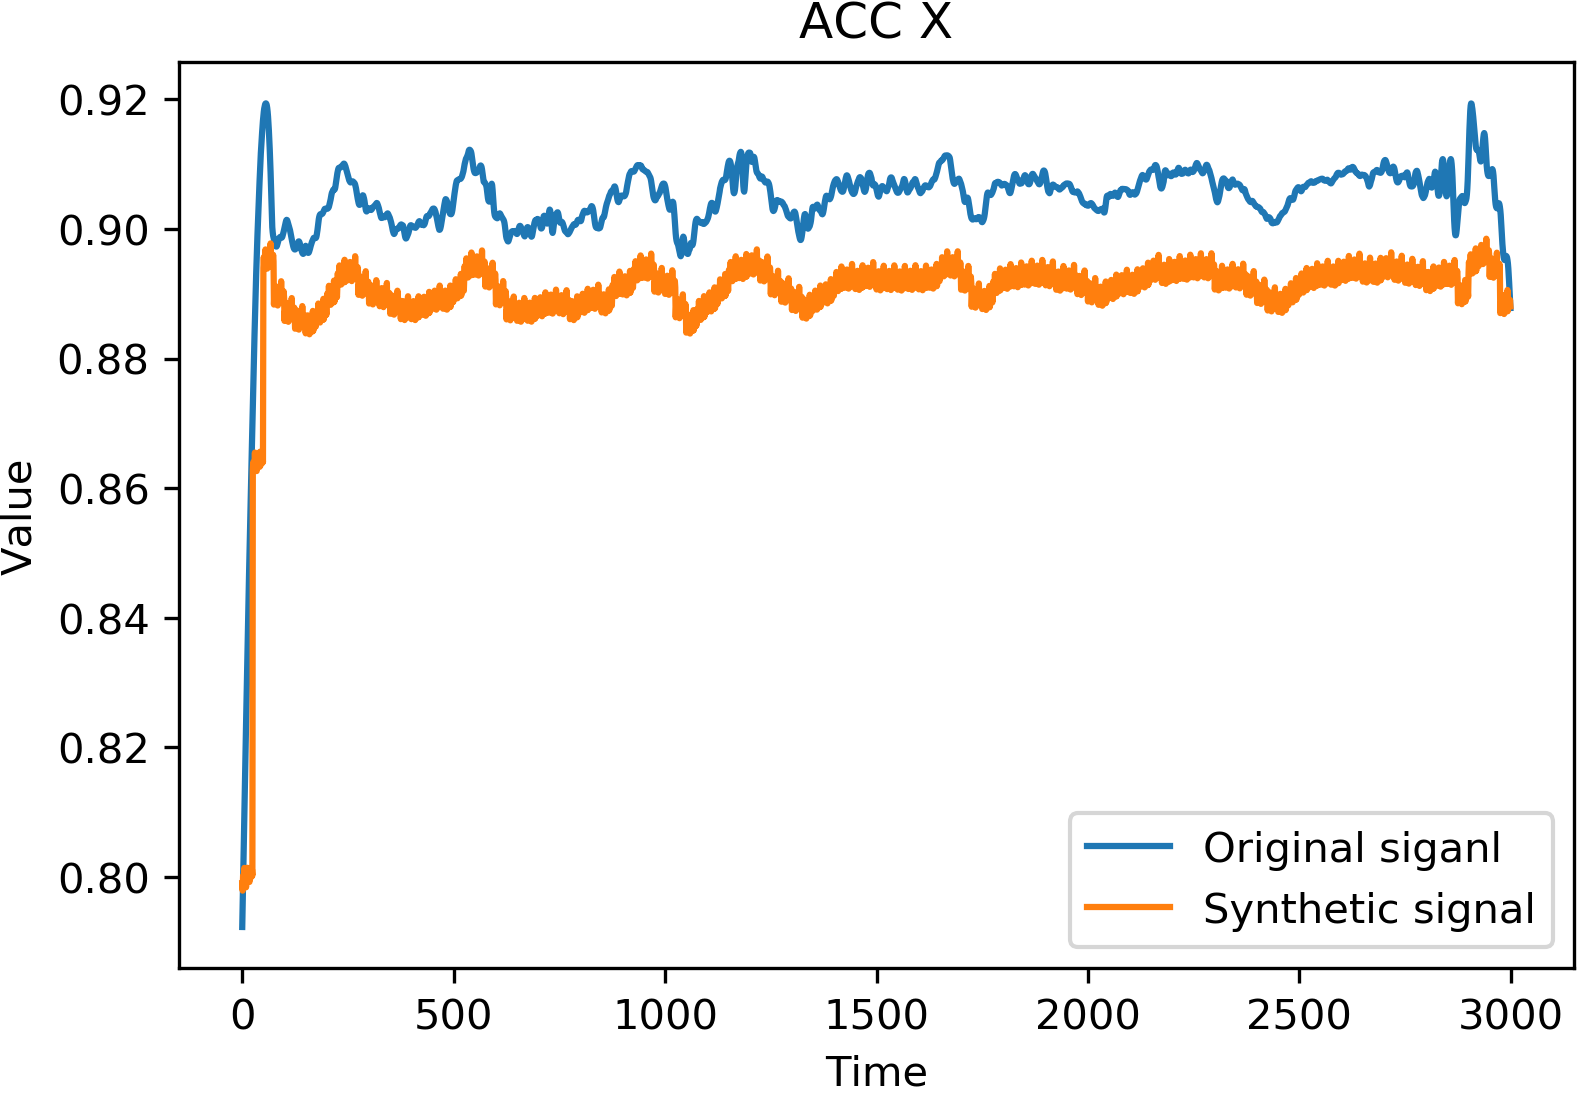
\includegraphics[width=.24\textwidth, height=2.8cm]{figs/sig_stress_ACC_X_acii2019_pres.png}\hfill
%   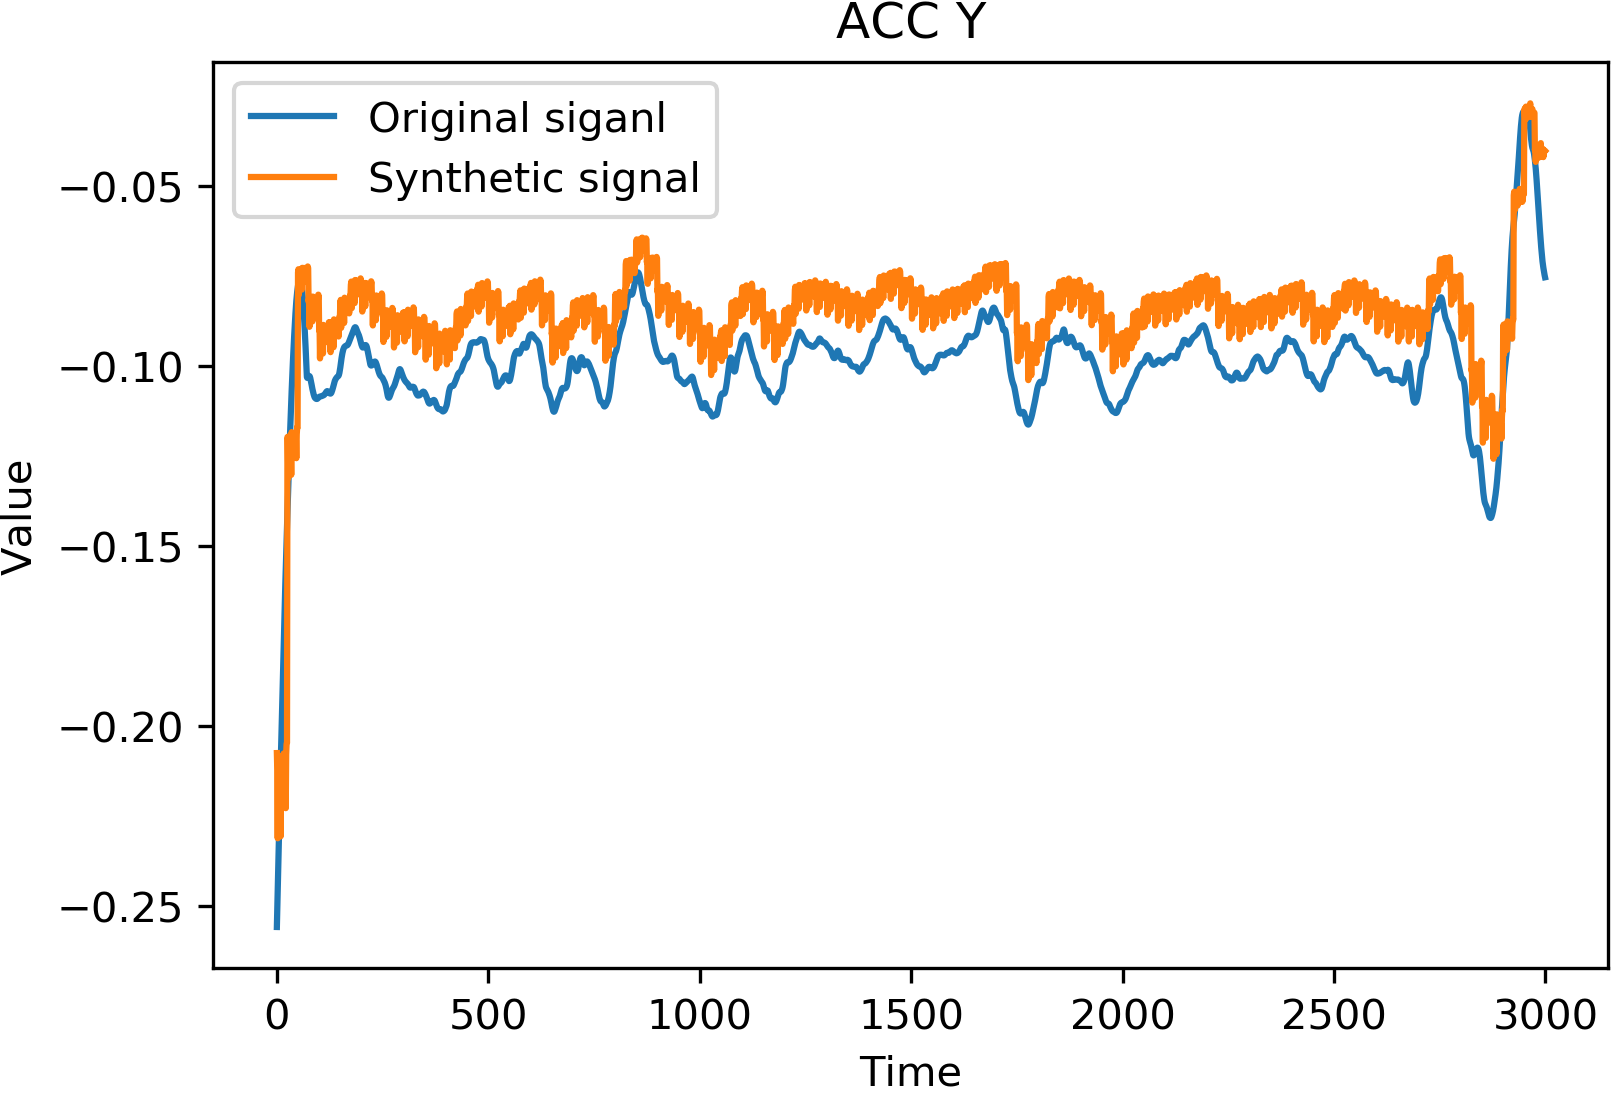
\includegraphics[width=.24\textwidth, height=2.8cm]{figs/sig_stress_ACC_Y_acii2019_pres.png}\hfill
%   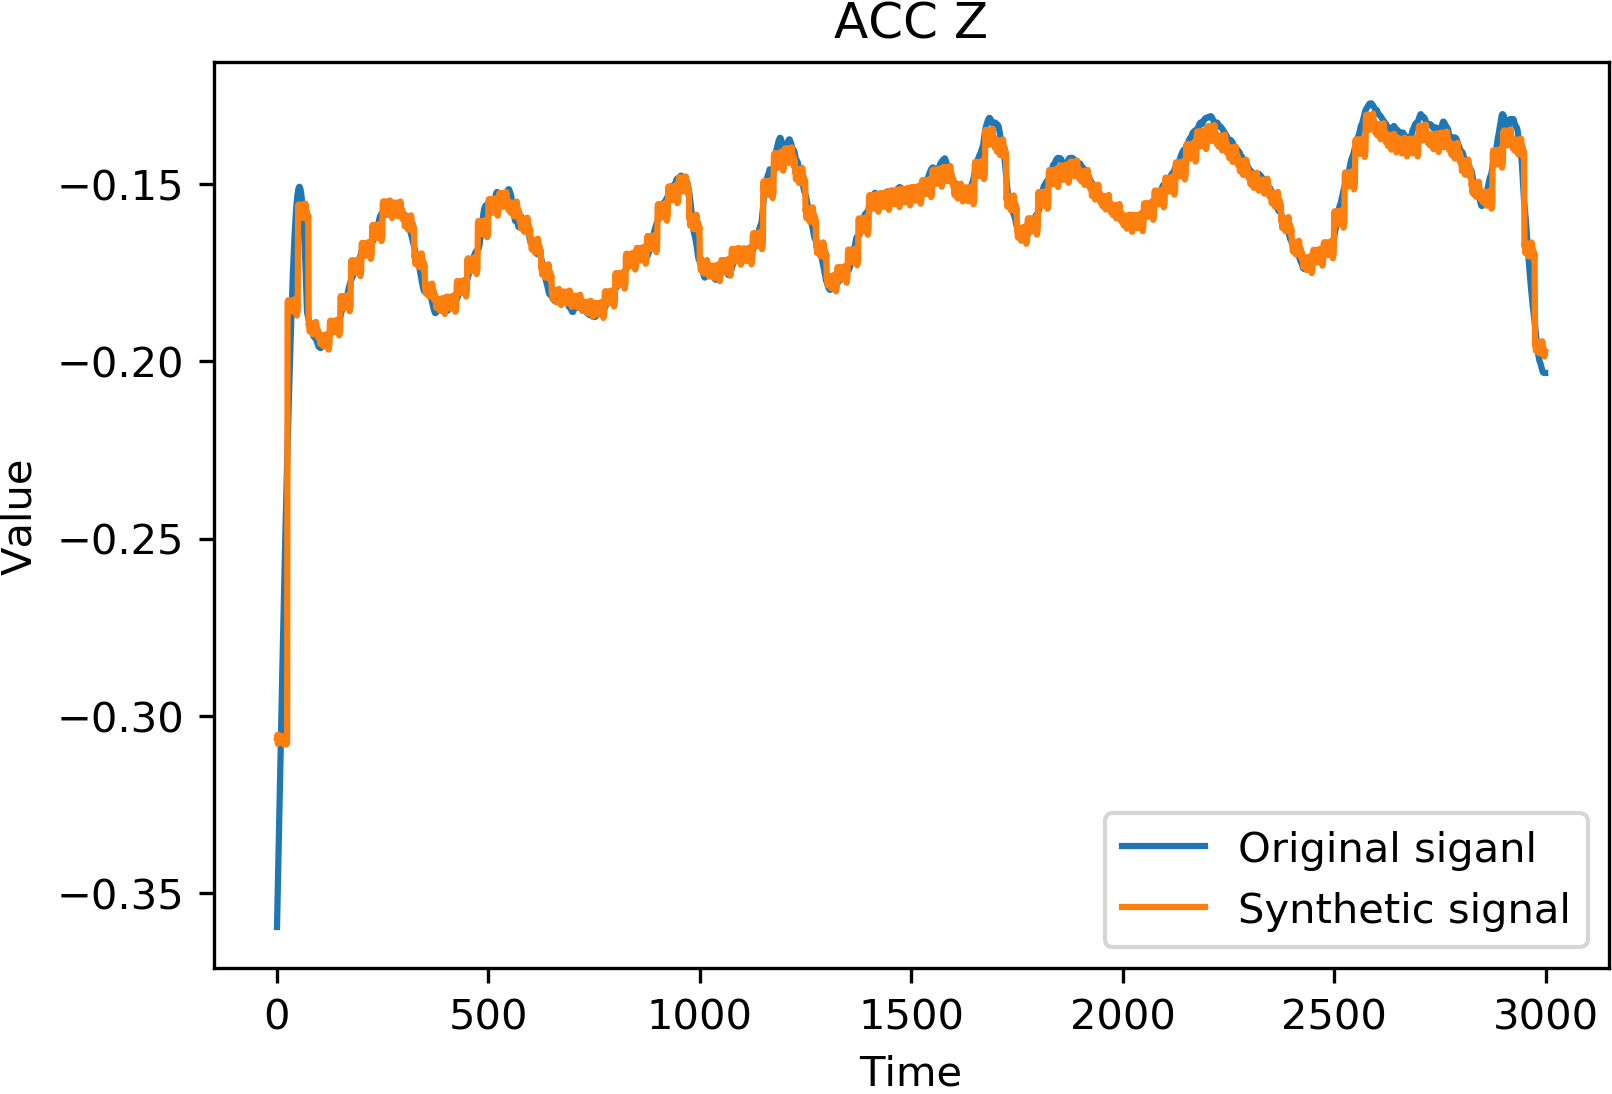
\includegraphics[width=.24\textwidth, height=2.8cm]{figs/sig_stress_ACC_Z_acii2019_pres.png}\hfill
%   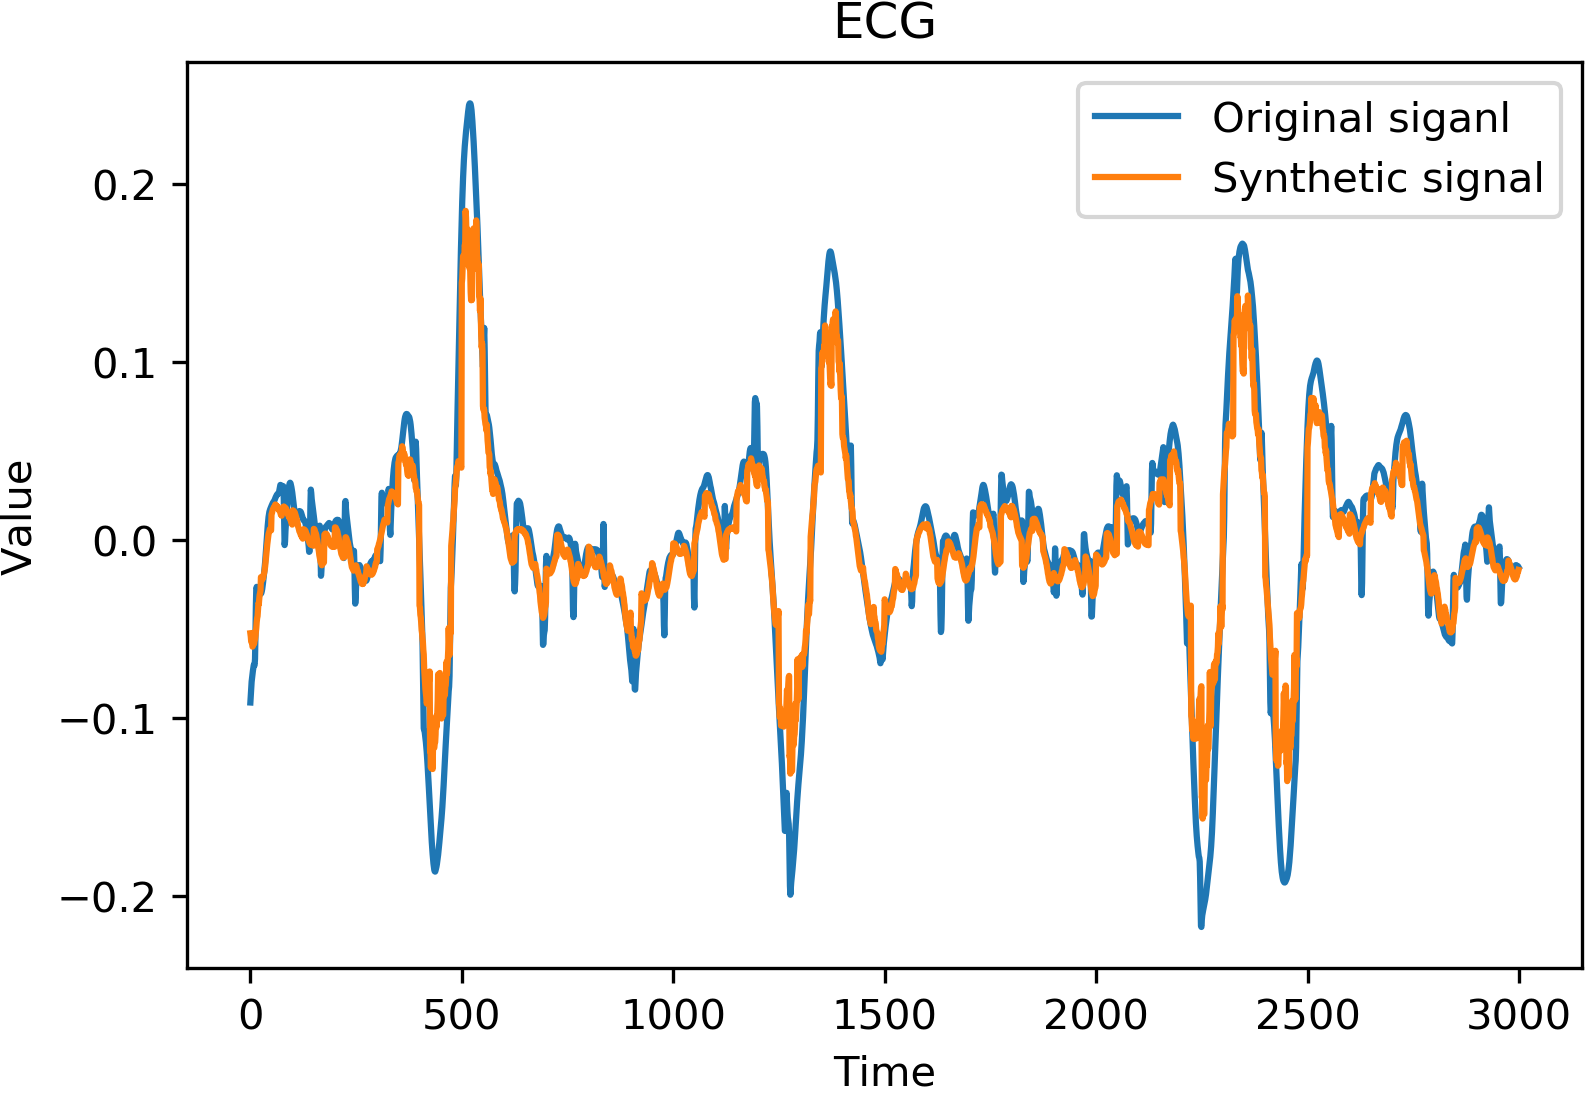
\includegraphics[width=.24\textwidth, height=2.8cm]{figs/sig_stress_ECG_acii2019_pres.png}\par
  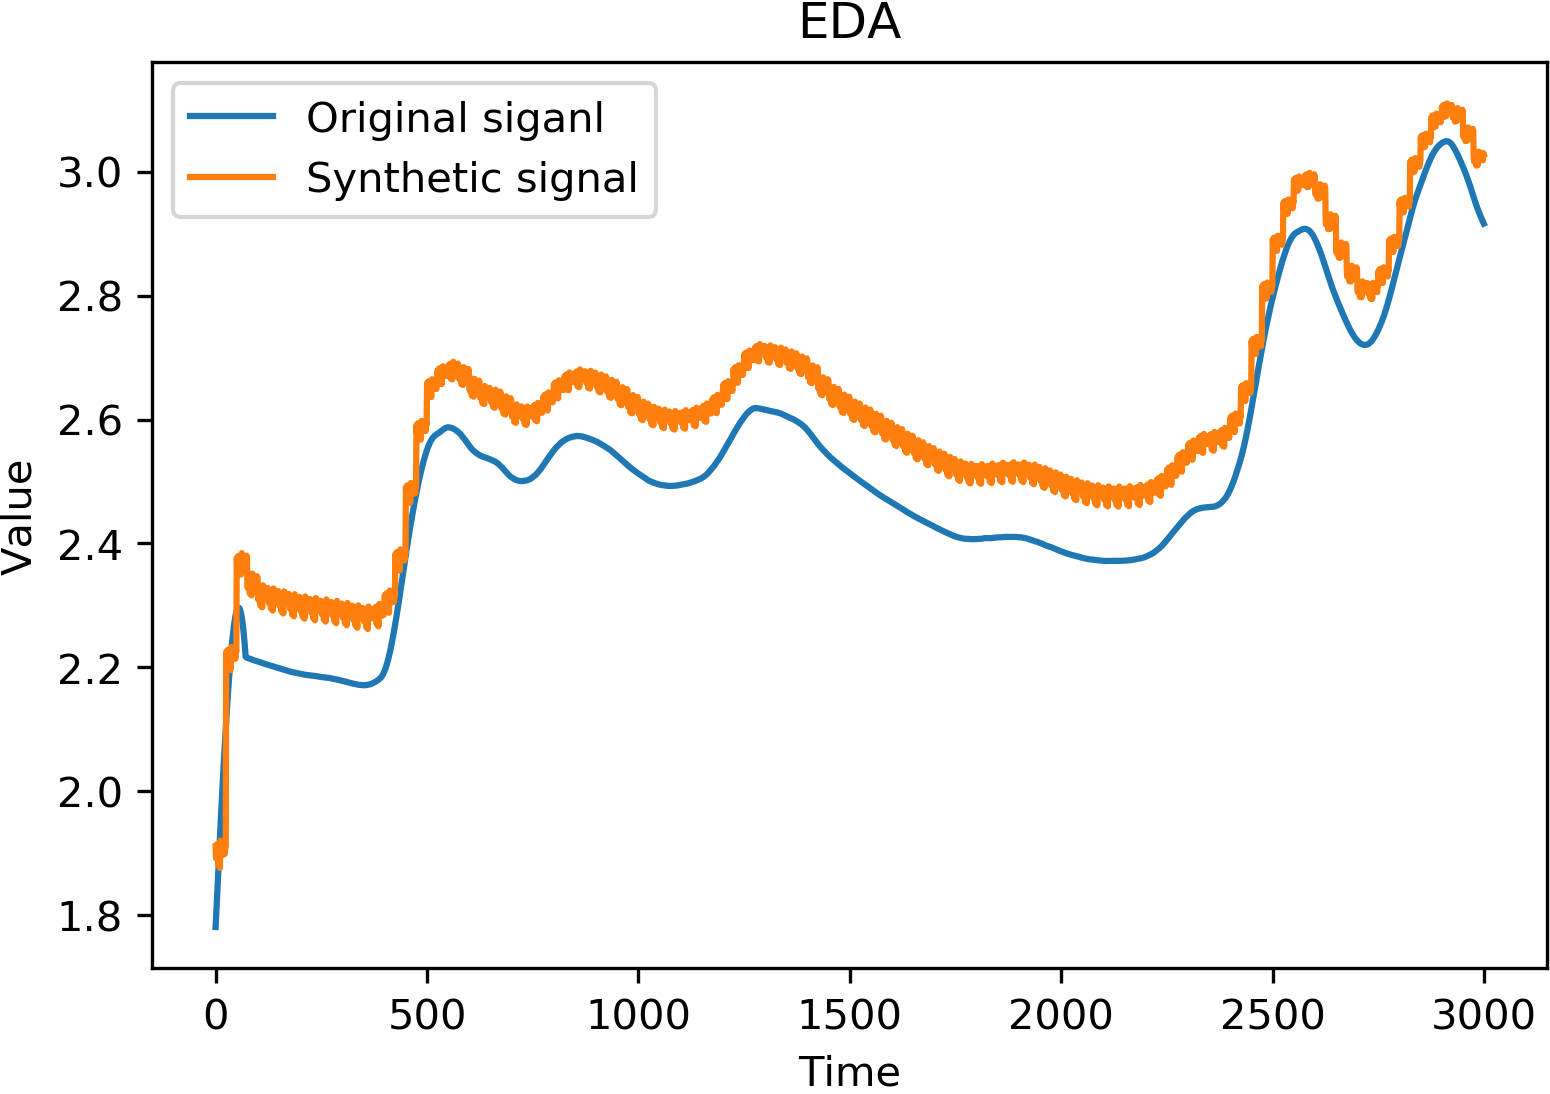
\includegraphics[width=.5\textwidth, height=5cm]{figs/sig_stress_EDA_acii2019_pres.png}\hfill
%   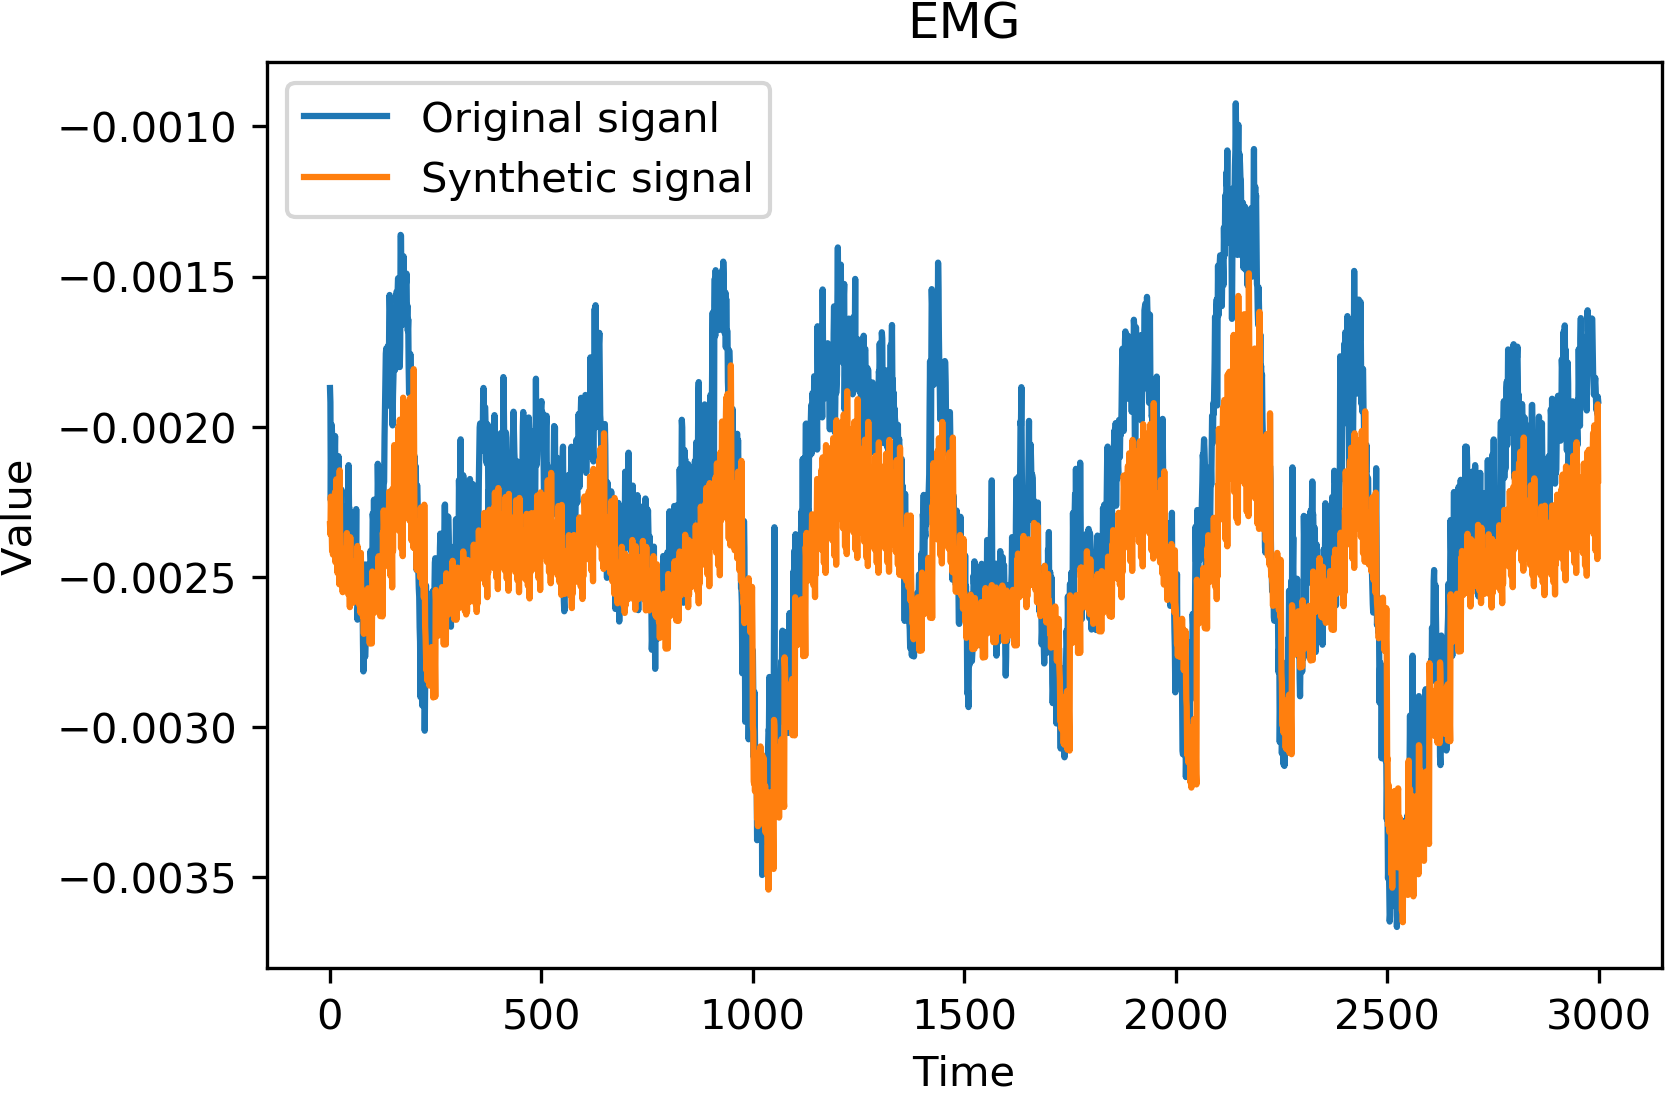
\includegraphics[width=.24\textwidth, height=2.8cm]{figs/sig_stress_EMG_acii2019_pres.png}
%   \hfill
%   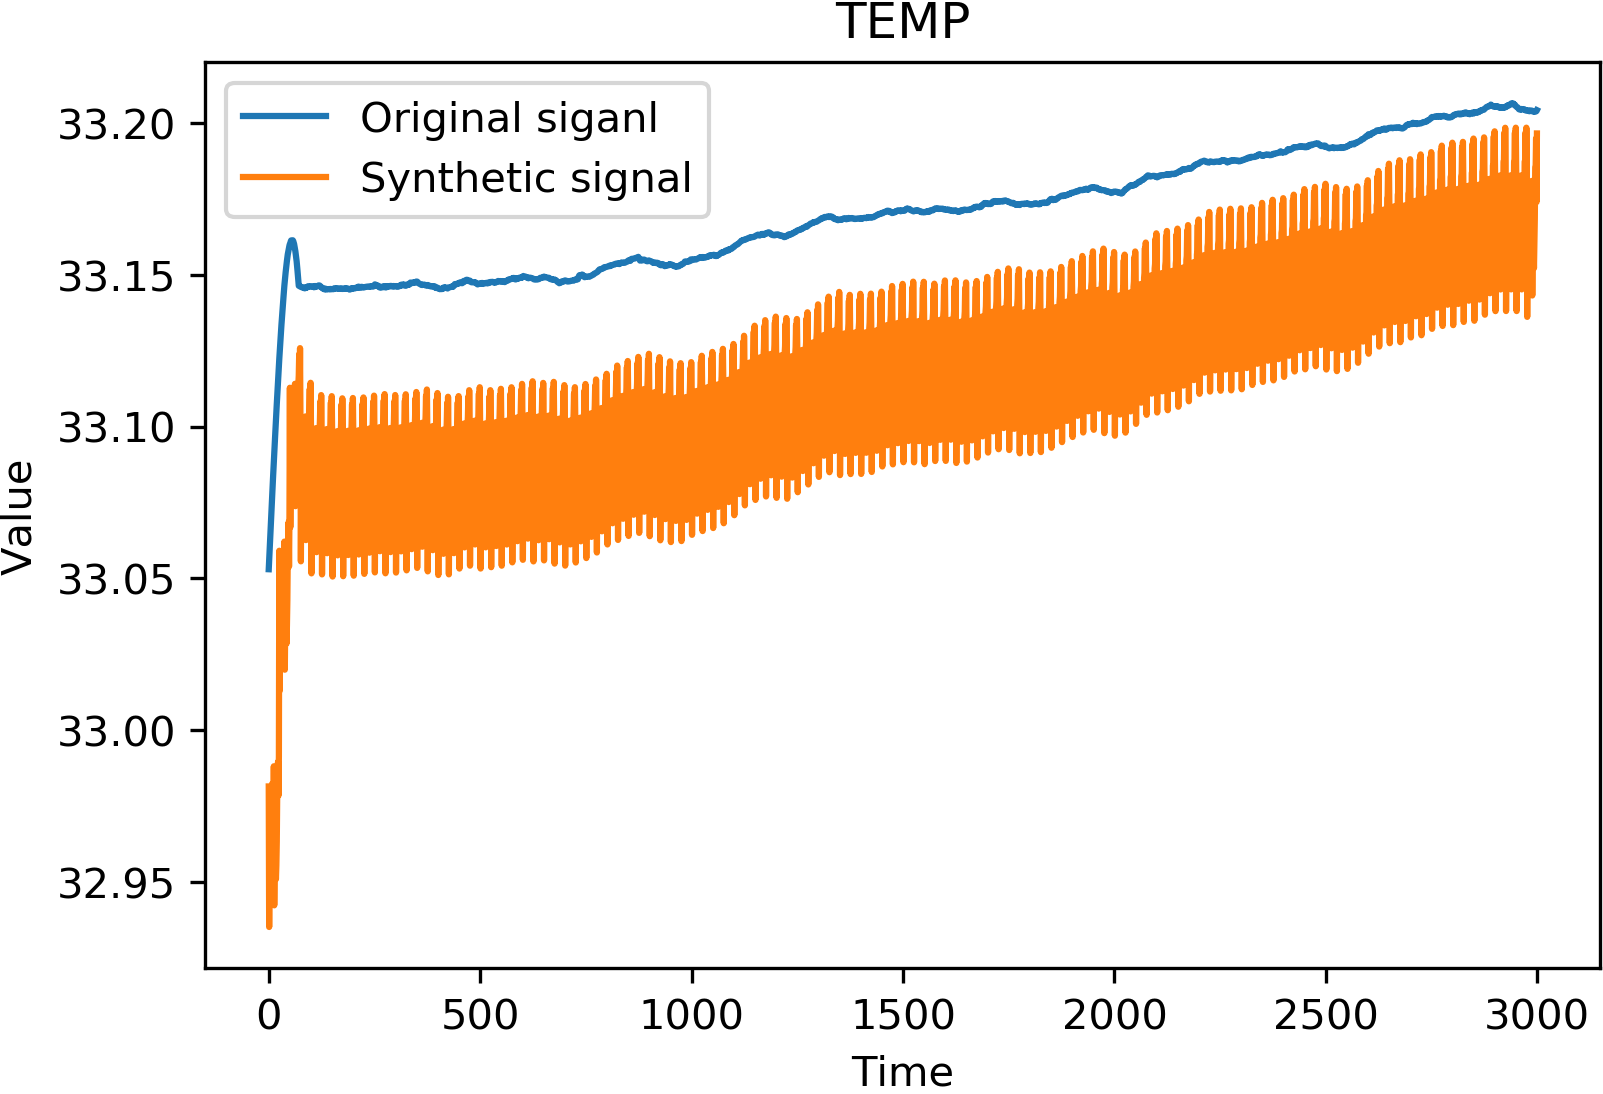
\includegraphics[width=.24\textwidth, height=2.8cm]{figs/sig_stress_Temp_acii2019_pres.png}\hfill
%   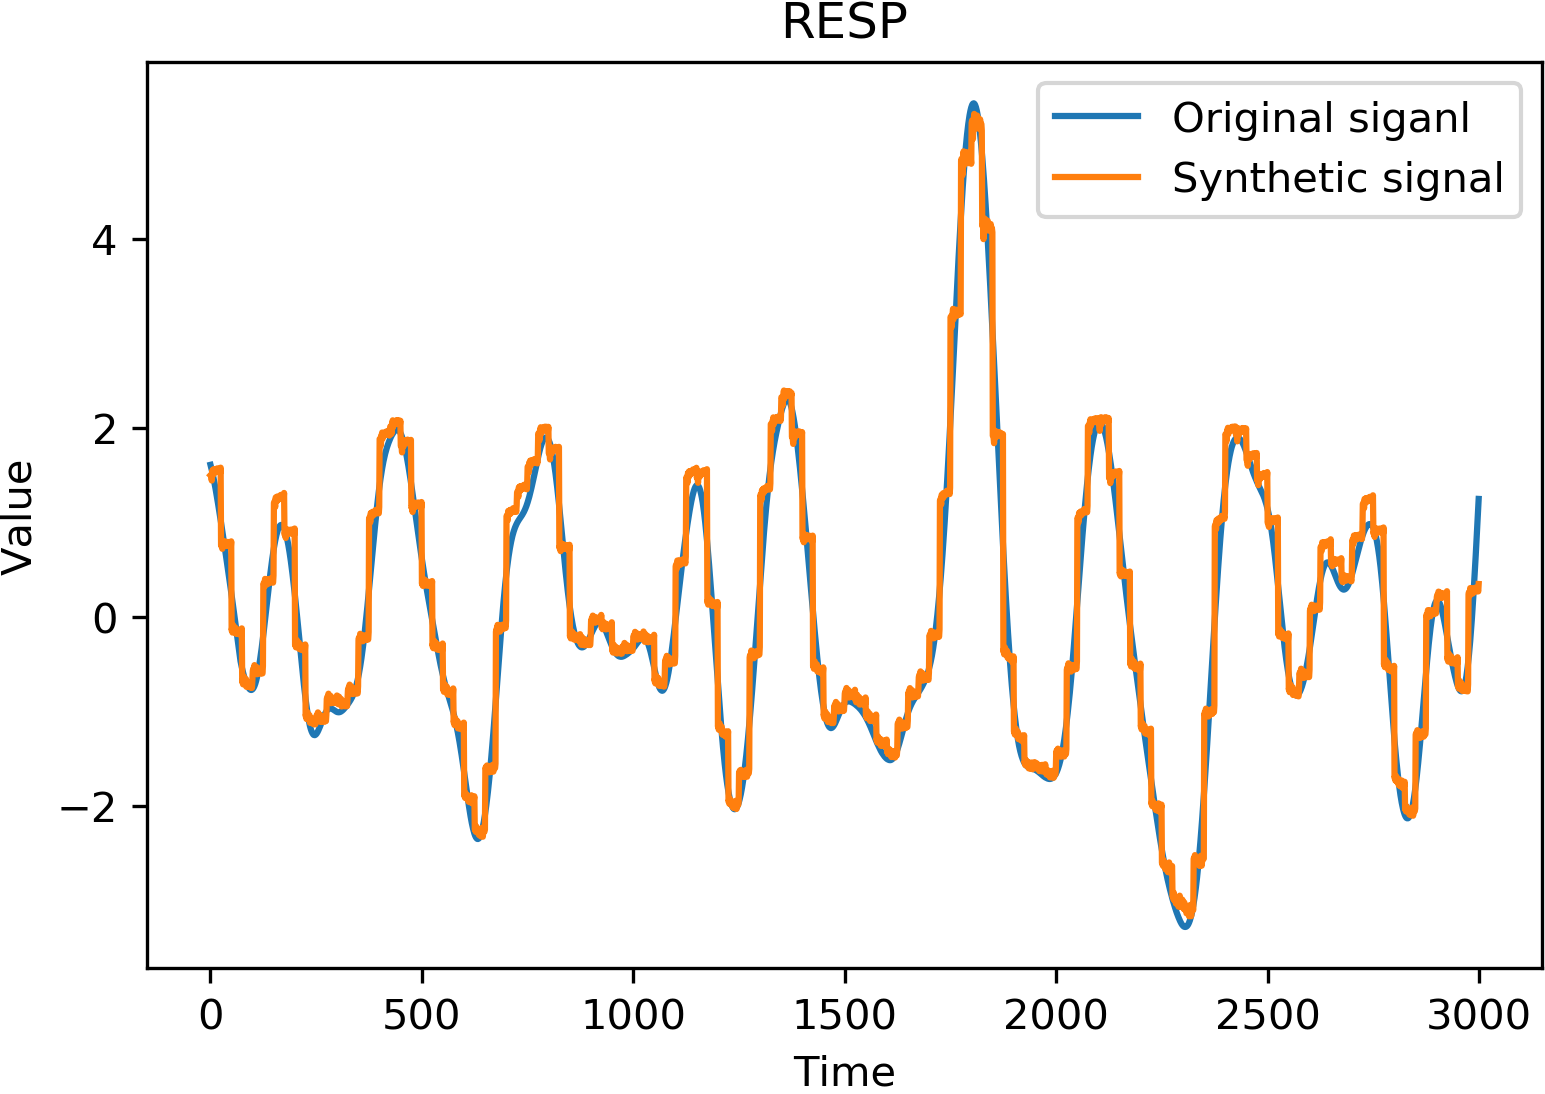
\includegraphics[width=.24\textwidth, height=2.8cm]{figs/sig_stress_Resp_acii2019_pres.png}\hfill

  \label{sig_plot}
\end{figure}

\end{frame}



\begin{frame}
\frametitle{Sample Signals (Original and Synthesis)}

% \section{Experimental Design and Results}
\begin{figure}
  \centering
  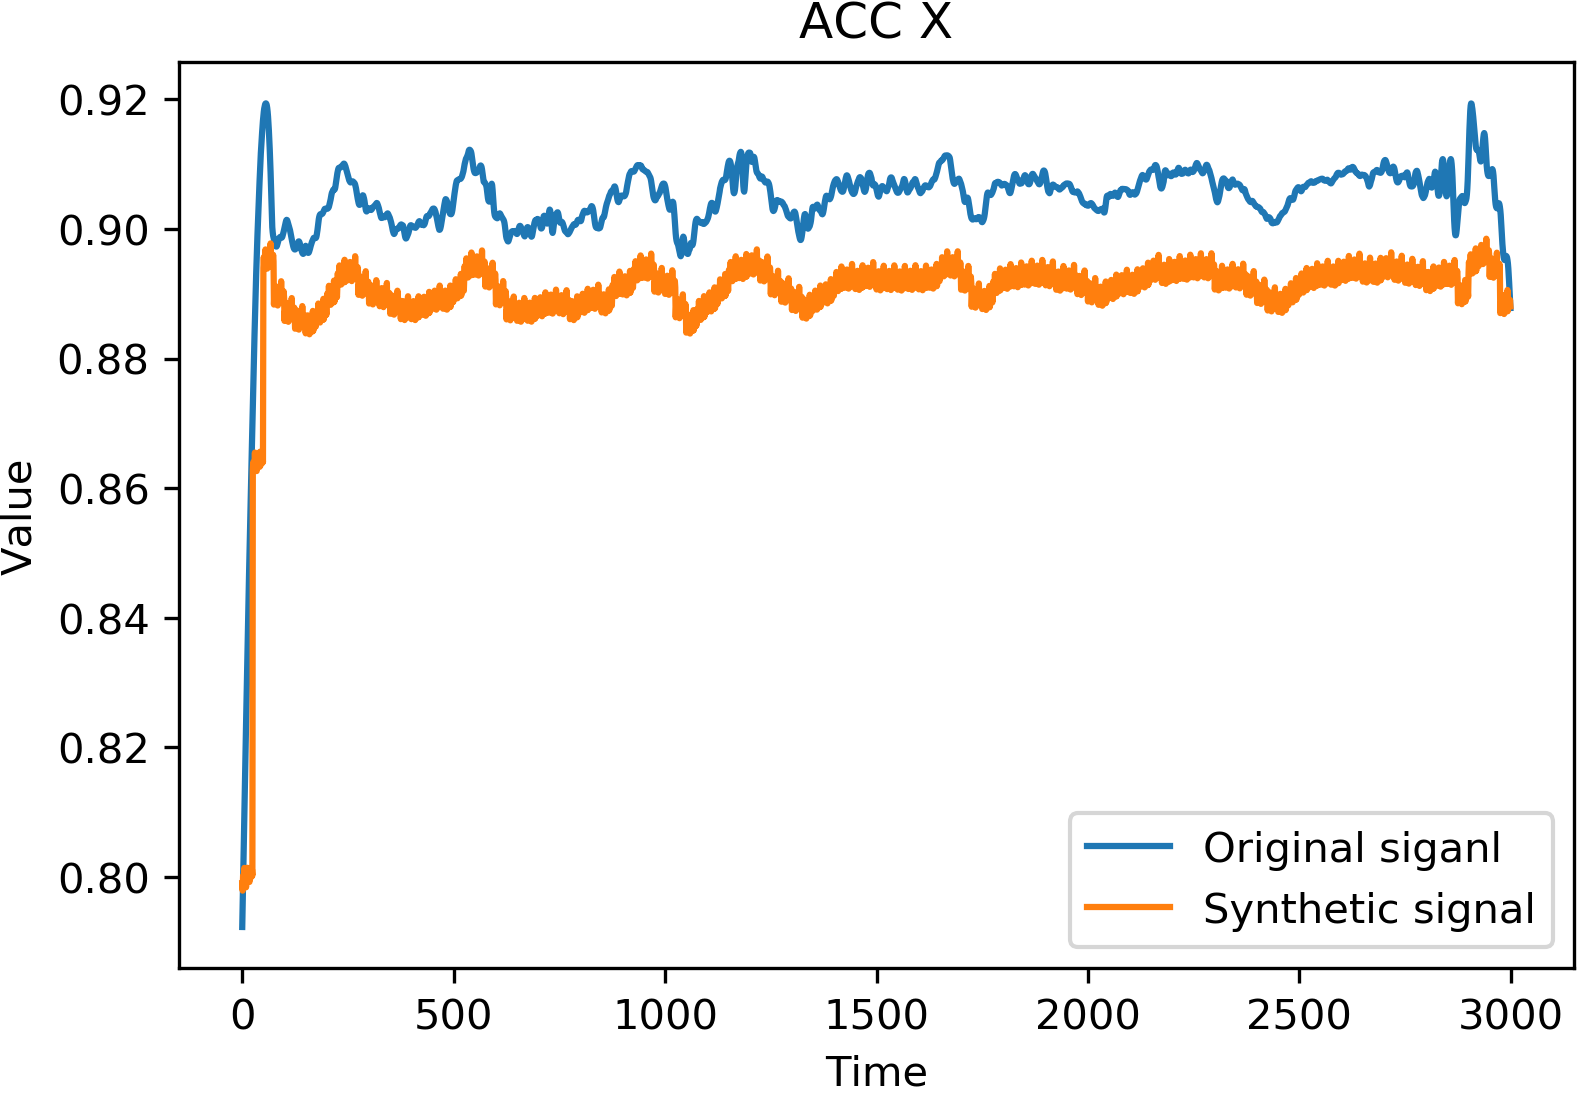
\includegraphics[width=.24\textwidth, height=2.8cm]{figs/sig_stress_ACC_X_acii2019_pres.png}\hfill
  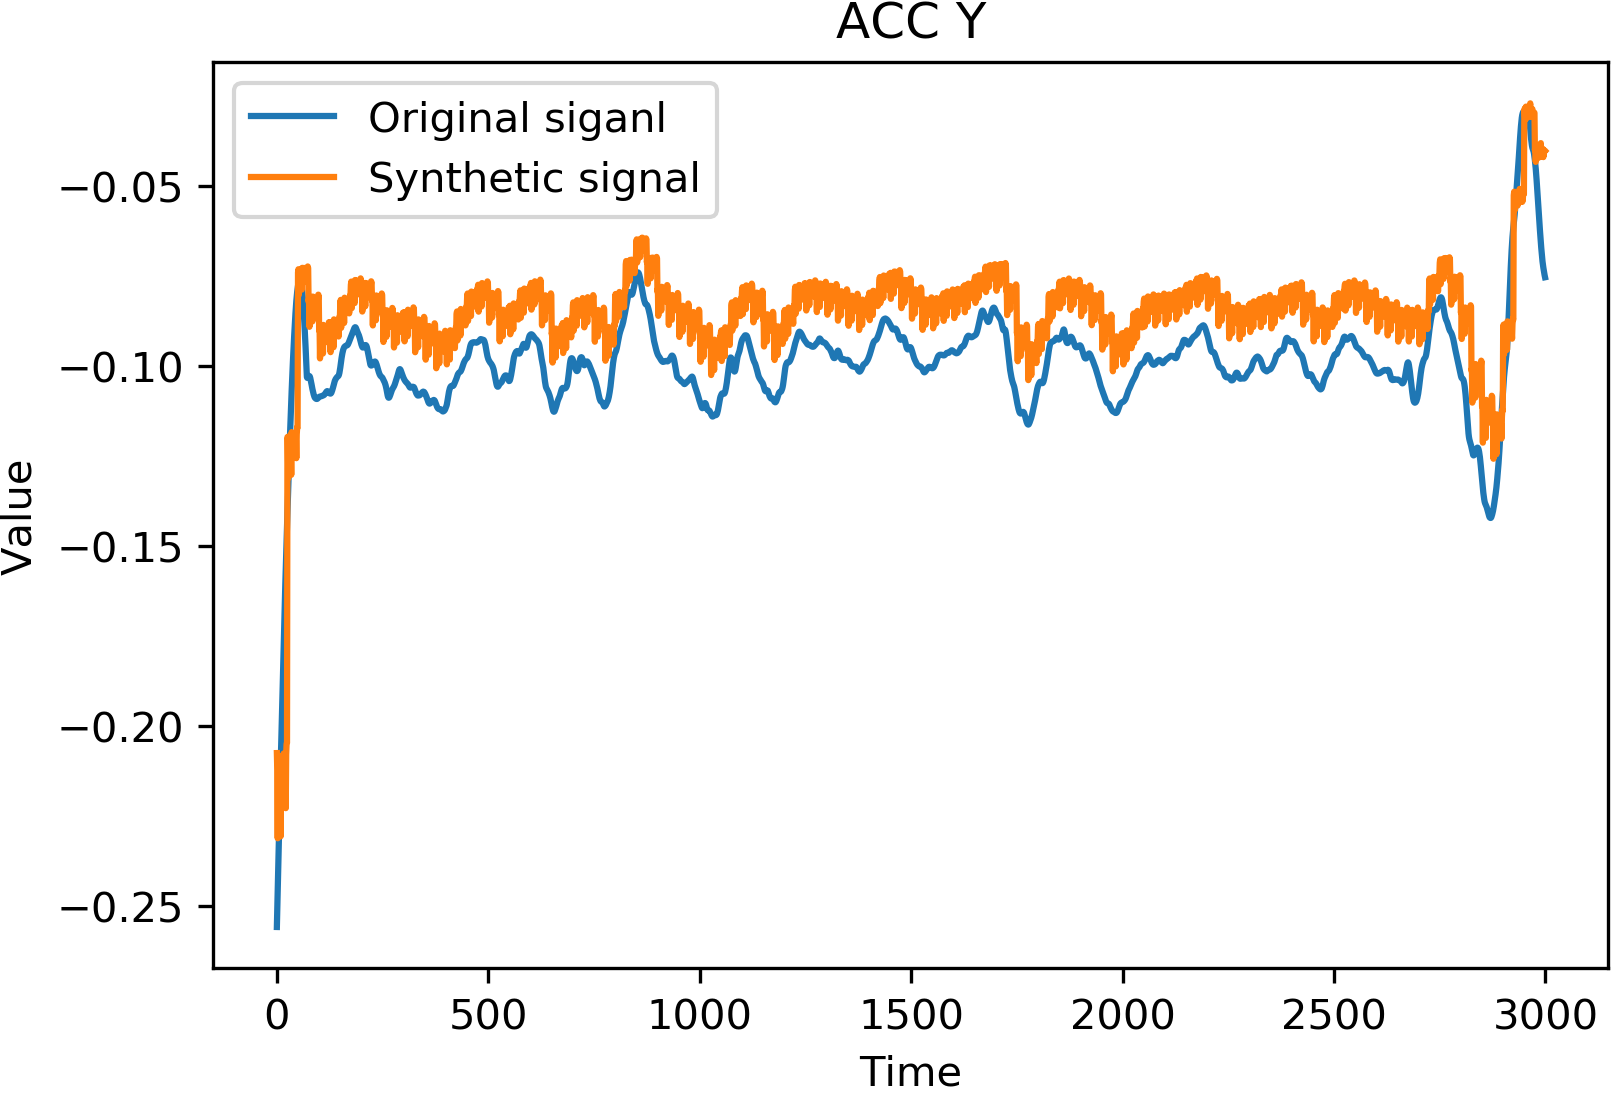
\includegraphics[width=.24\textwidth, height=2.8cm]{figs/sig_stress_ACC_Y_acii2019_pres.png}\hfill
  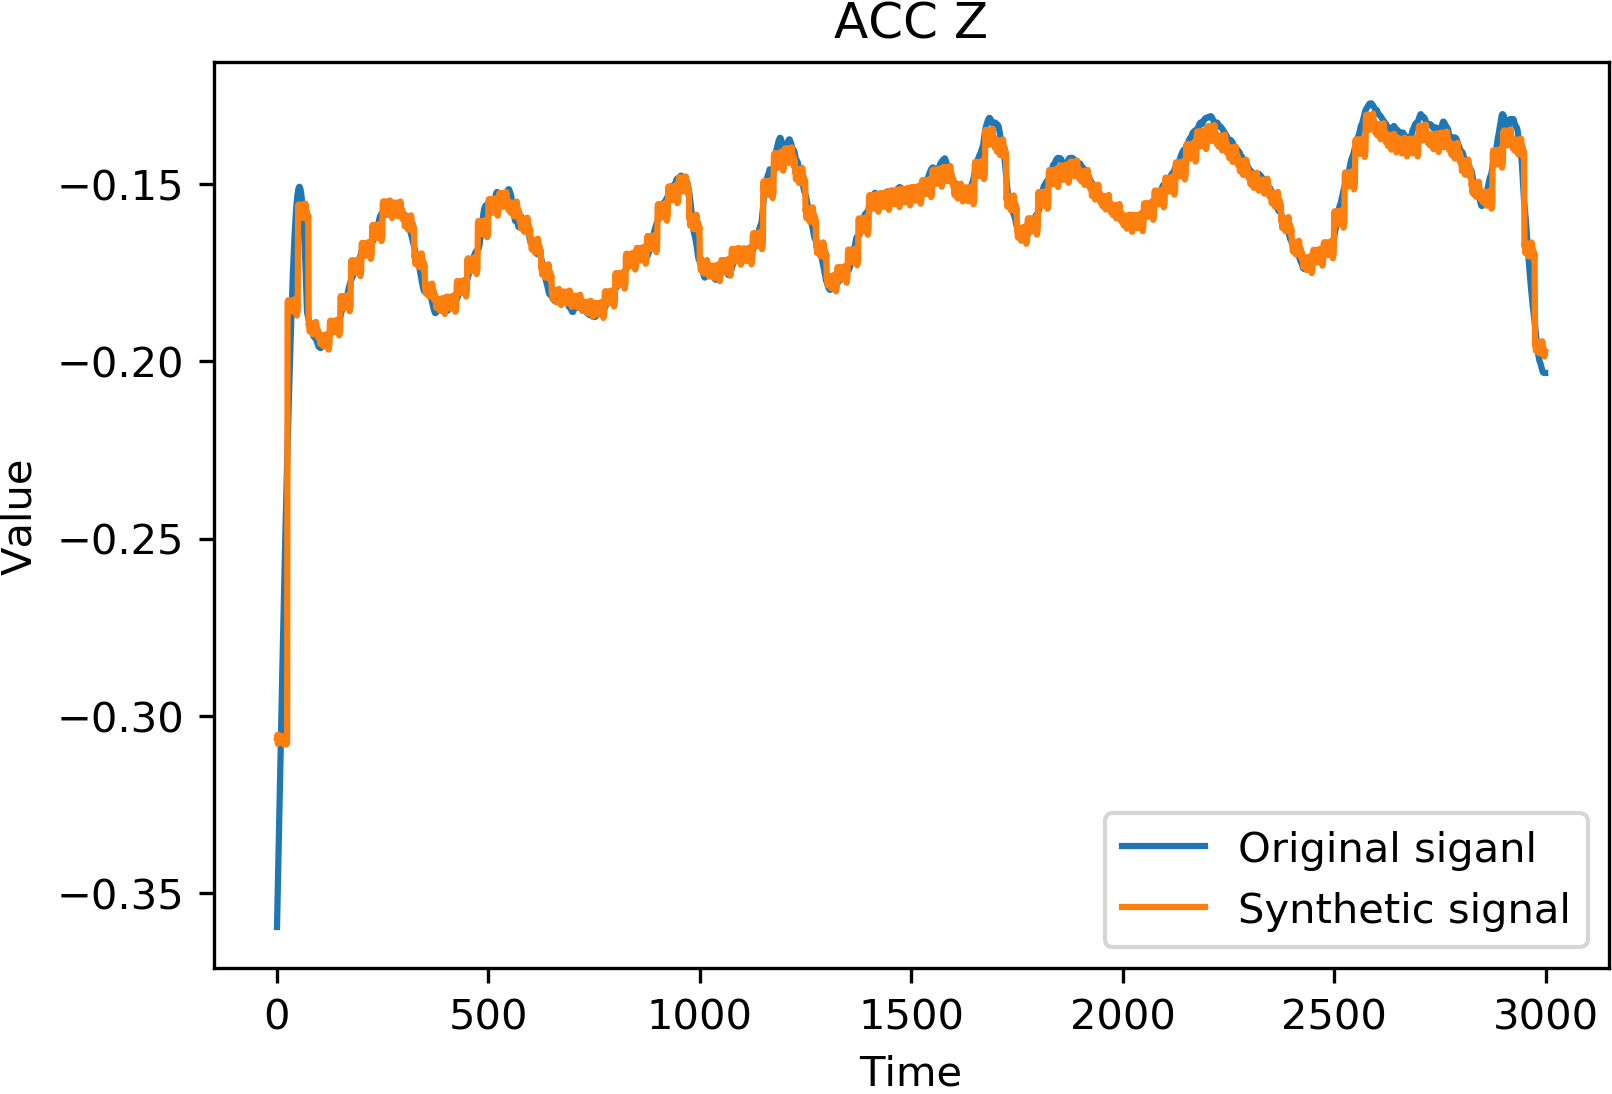
\includegraphics[width=.24\textwidth, height=2.8cm]{figs/sig_stress_ACC_Z_acii2019_pres.png}\hfill
  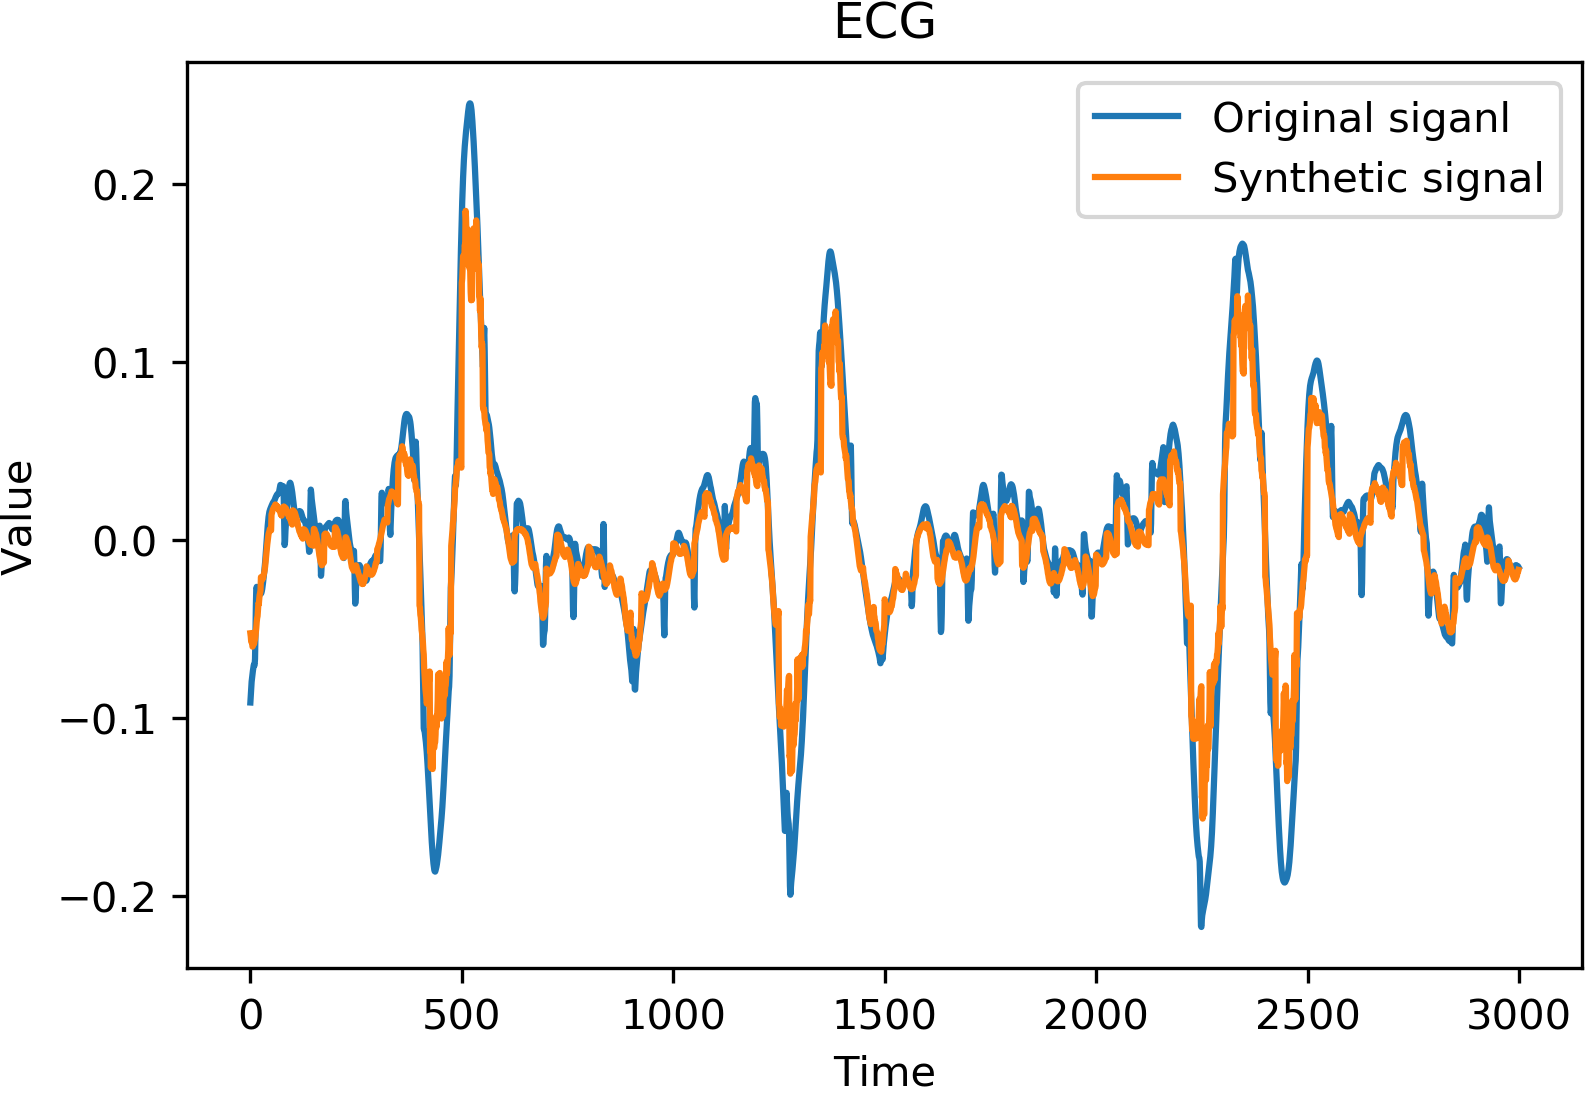
\includegraphics[width=.24\textwidth, height=2.8cm]{figs/sig_stress_ECG_acii2019_pres.png}\par
  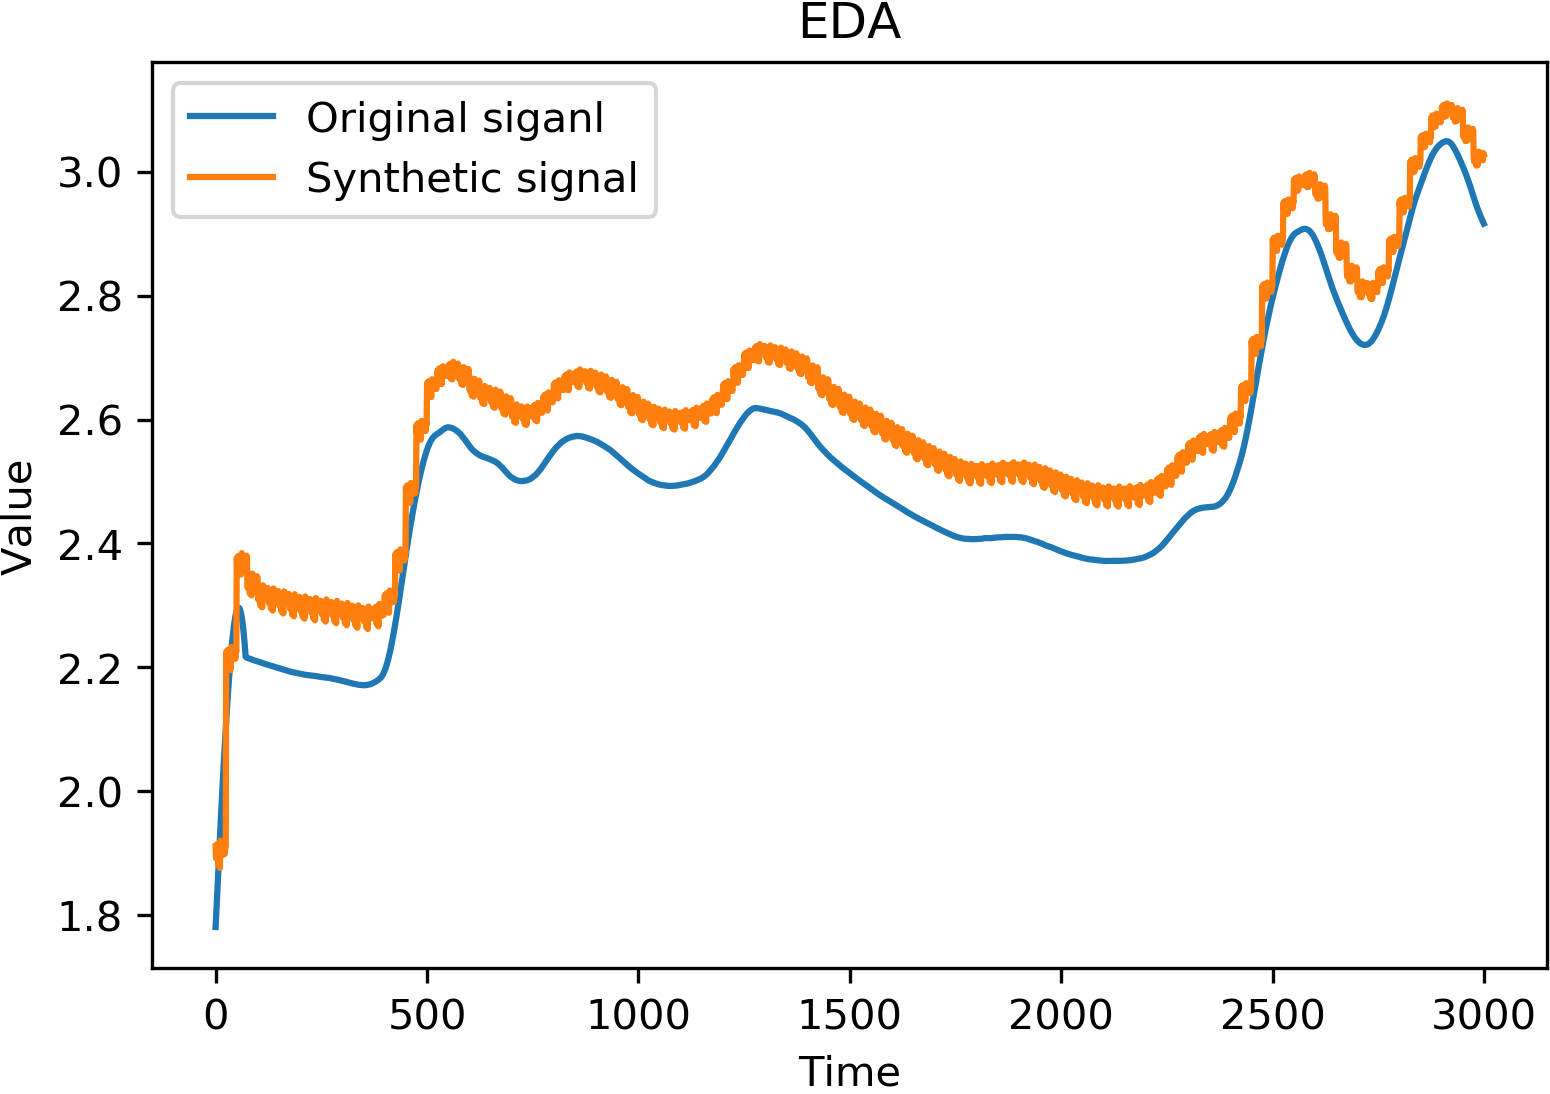
\includegraphics[width=.24\textwidth, height=2.8cm]{figs/sig_stress_EDA_acii2019_pres.png}\hfill
  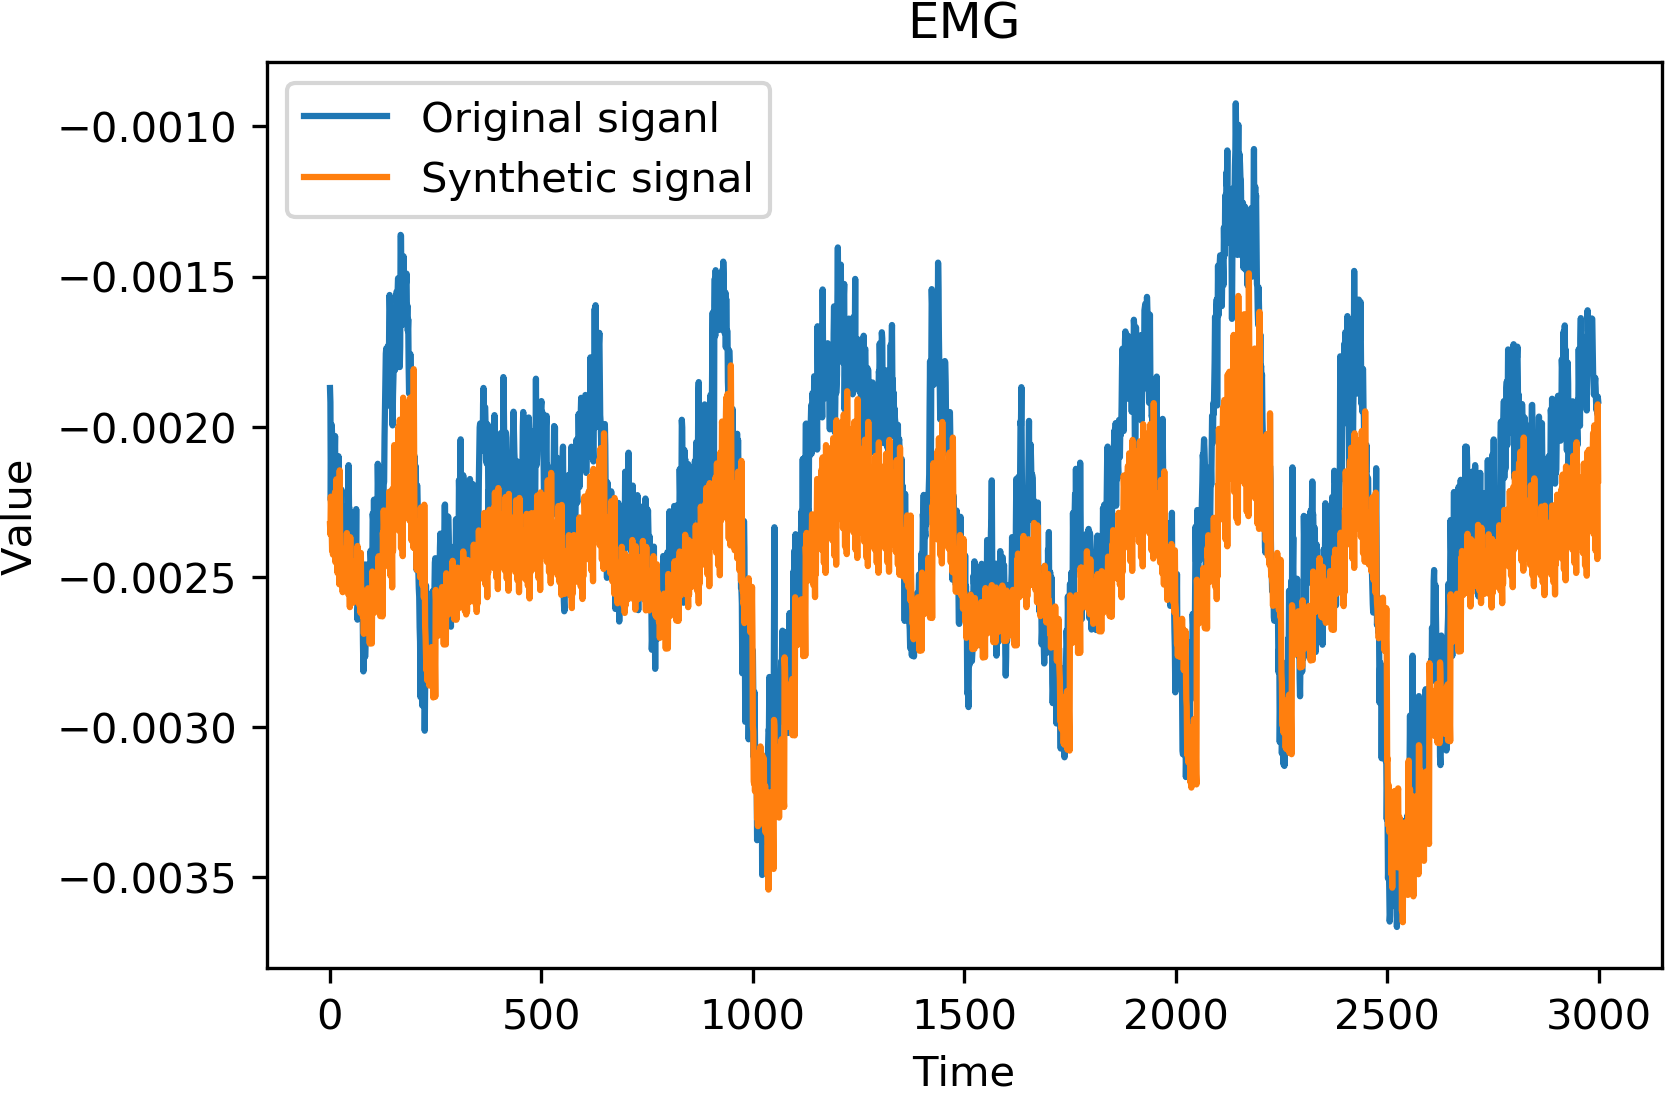
\includegraphics[width=.24\textwidth, height=2.8cm]{figs/sig_stress_EMG_acii2019_pres.png}
  \hfill
  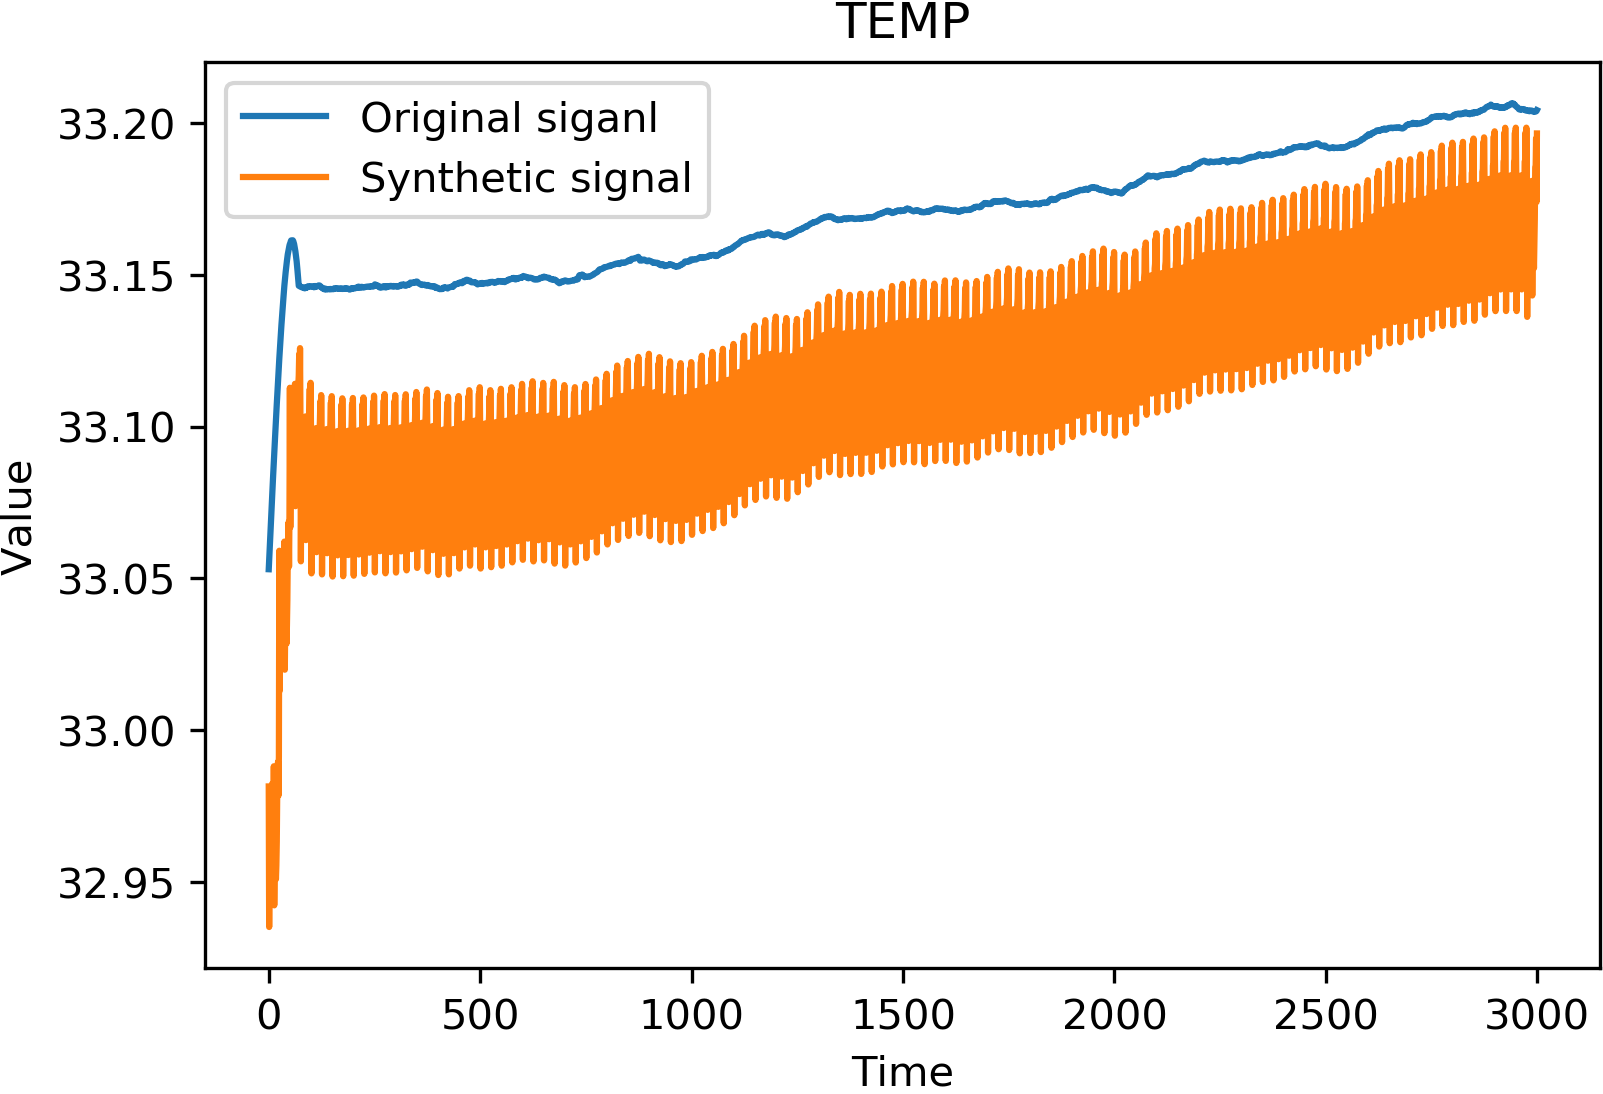
\includegraphics[width=.24\textwidth, height=2.8cm]{figs/sig_stress_Temp_acii2019_pres.png}\hfill
  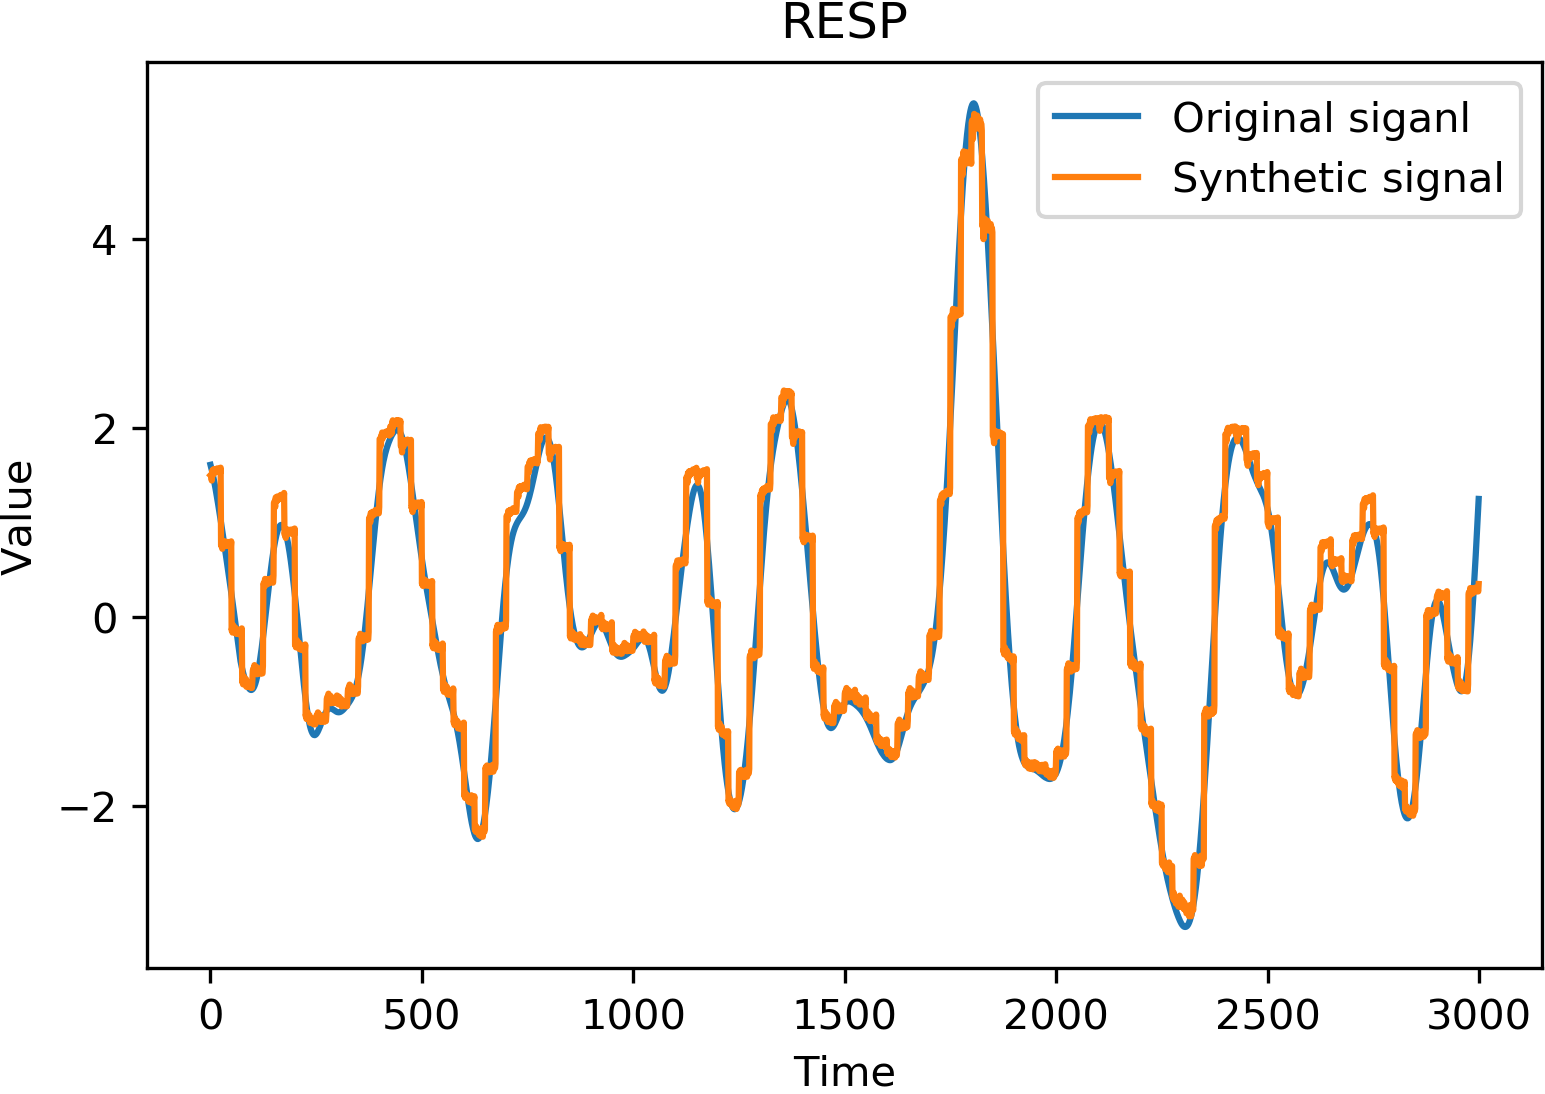
\includegraphics[width=.24\textwidth, height=2.8cm]{figs/sig_stress_Resp_acii2019_pres.png}\hfill

  \label{sig_plot}
\end{figure}

\end{frame}


\begin{frame}
\frametitle{Signal Distribution (Original and Synthesis)}

% Learned the distribution for all signals except EMG

\begin{figure}
  \centering
%   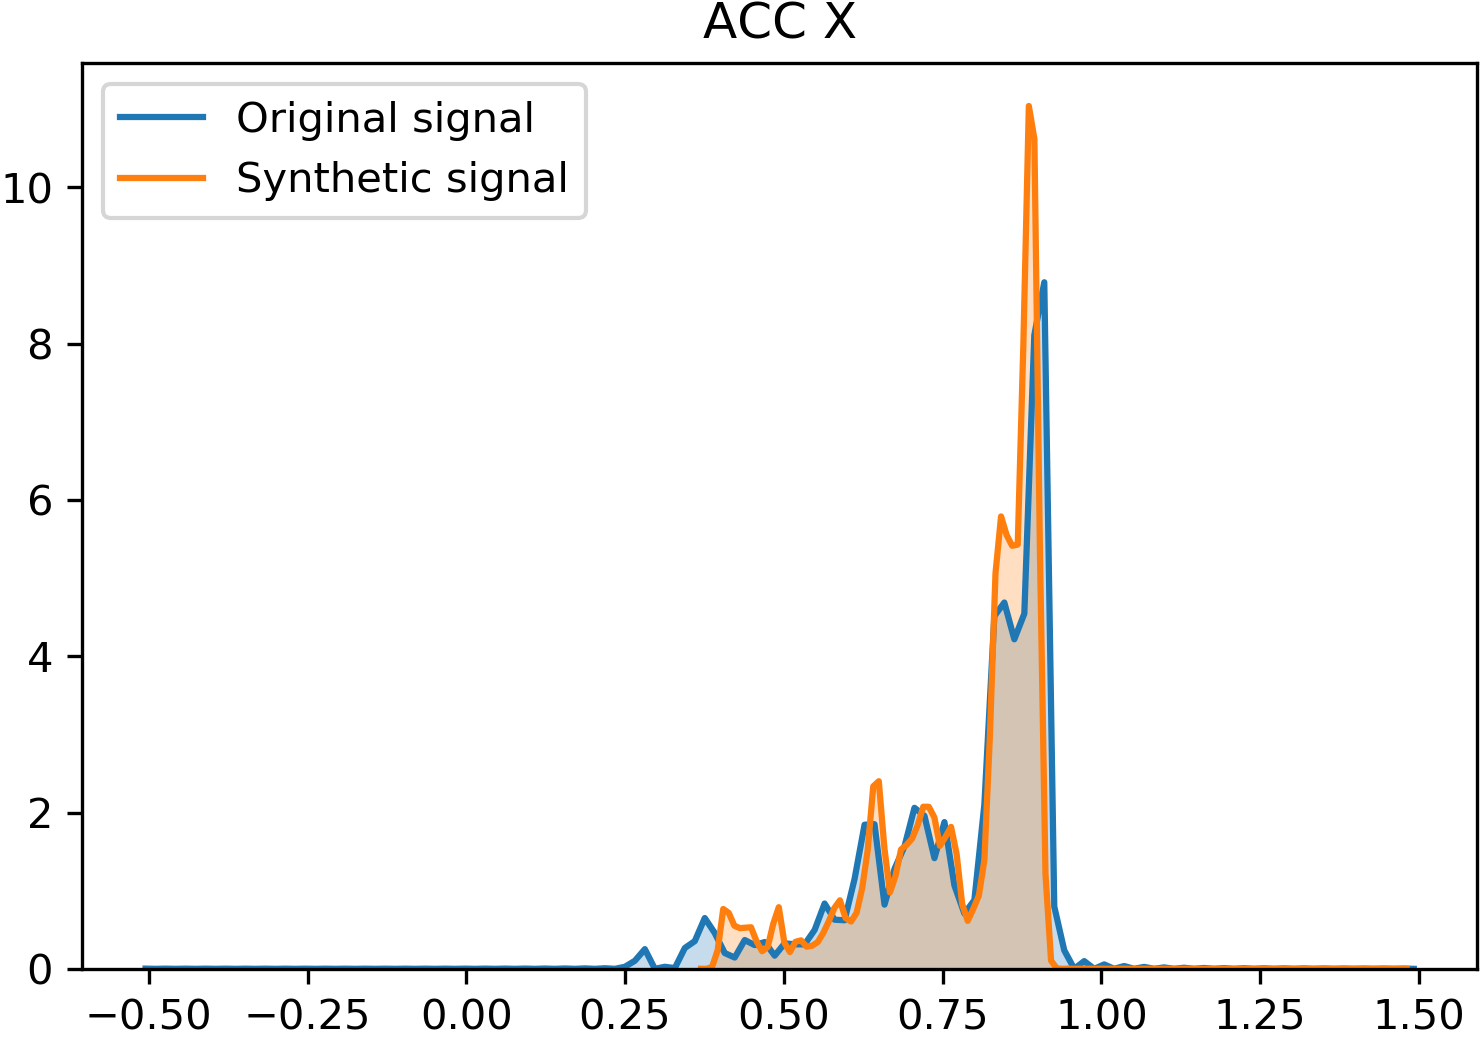
\includegraphics[width=.24\textwidth, height=2.8cm]{figs/dist_stress_ACC_X_acii2019_pres.png}\hfill
%   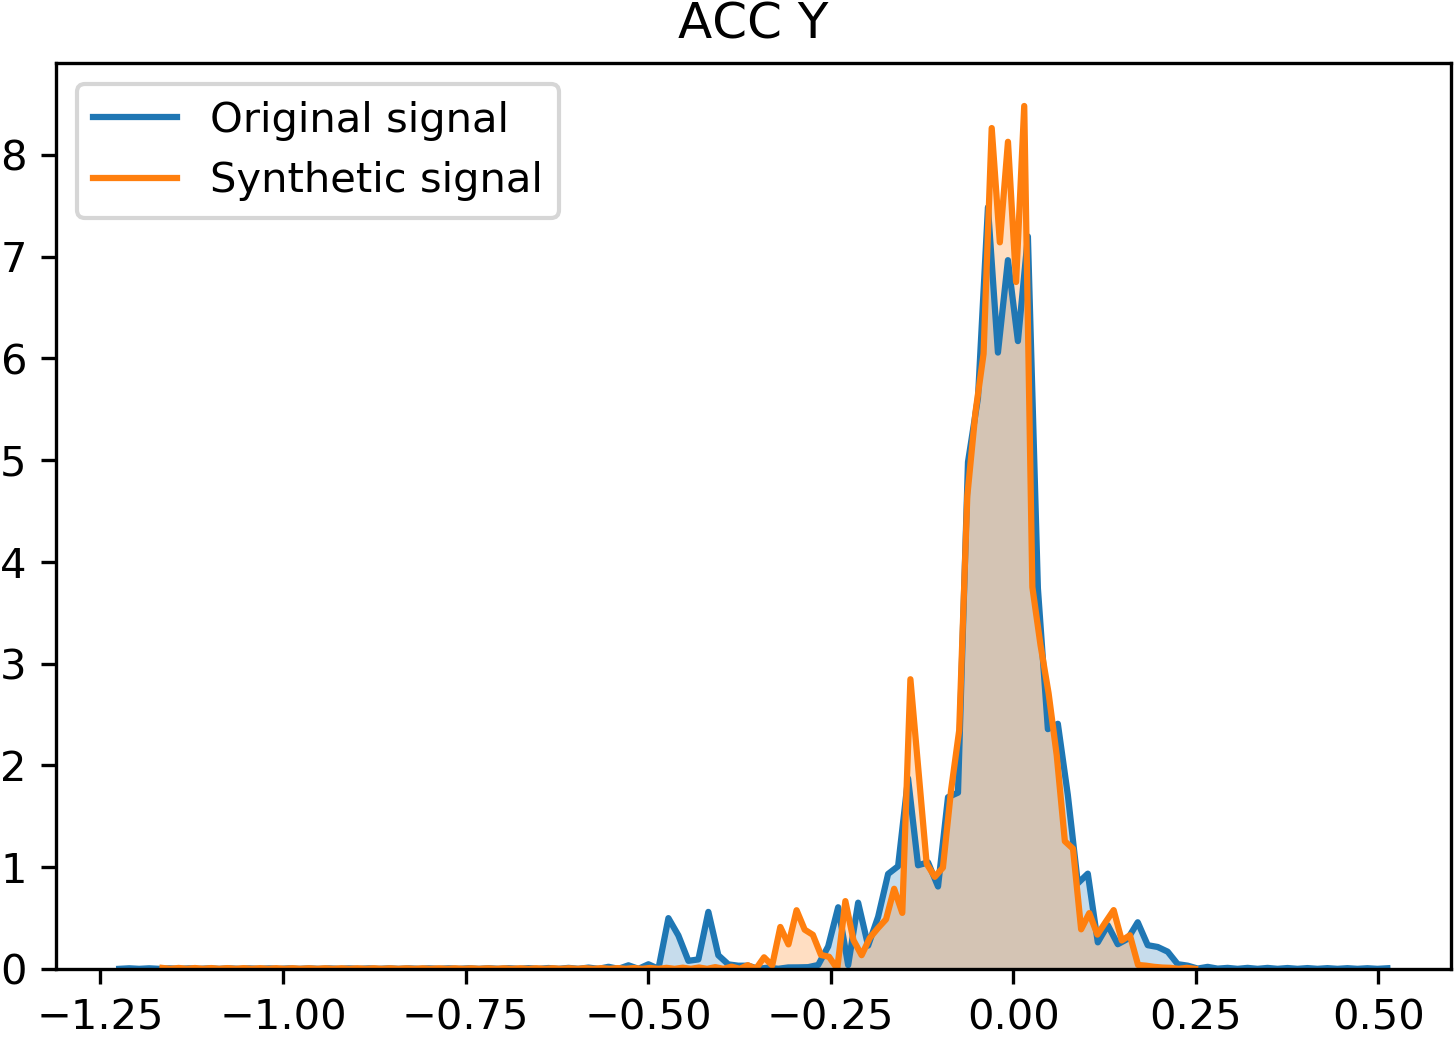
\includegraphics[width=.24\textwidth, height=2.8cm]{figs/dist_stress_ACC_Y_acii2019_pres.png}\hfill
%   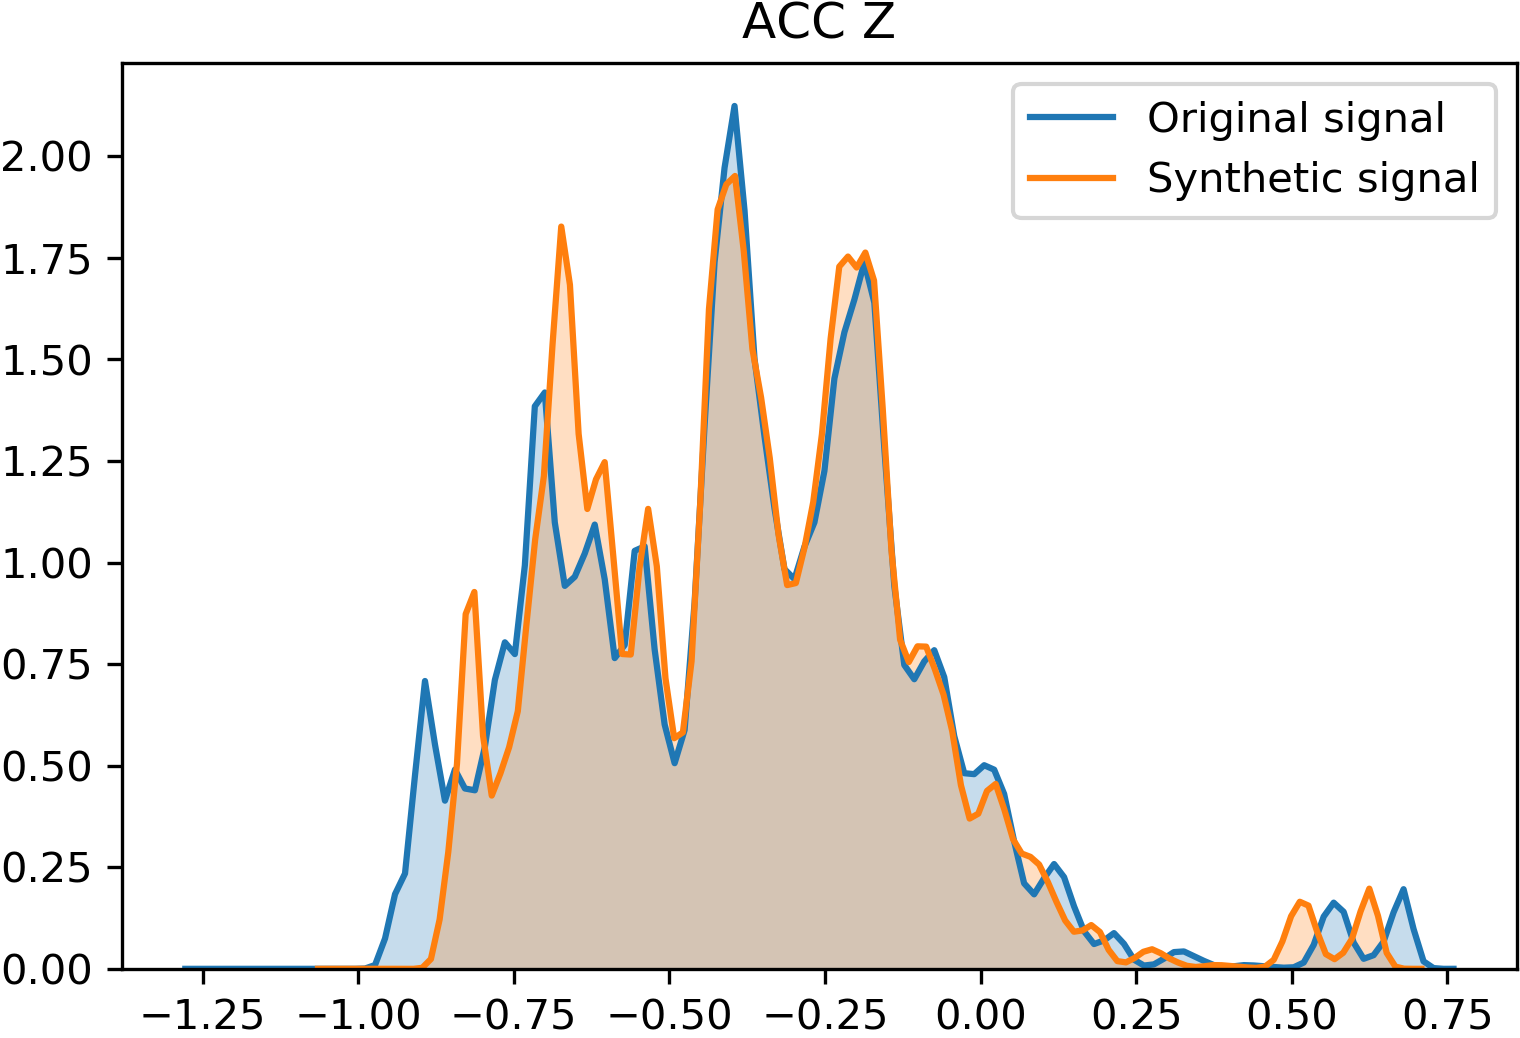
\includegraphics[width=.24\textwidth, height=2.8cm]{figs/dist_stress_ACC_Z_acii2019_pres.png}\hfill
%   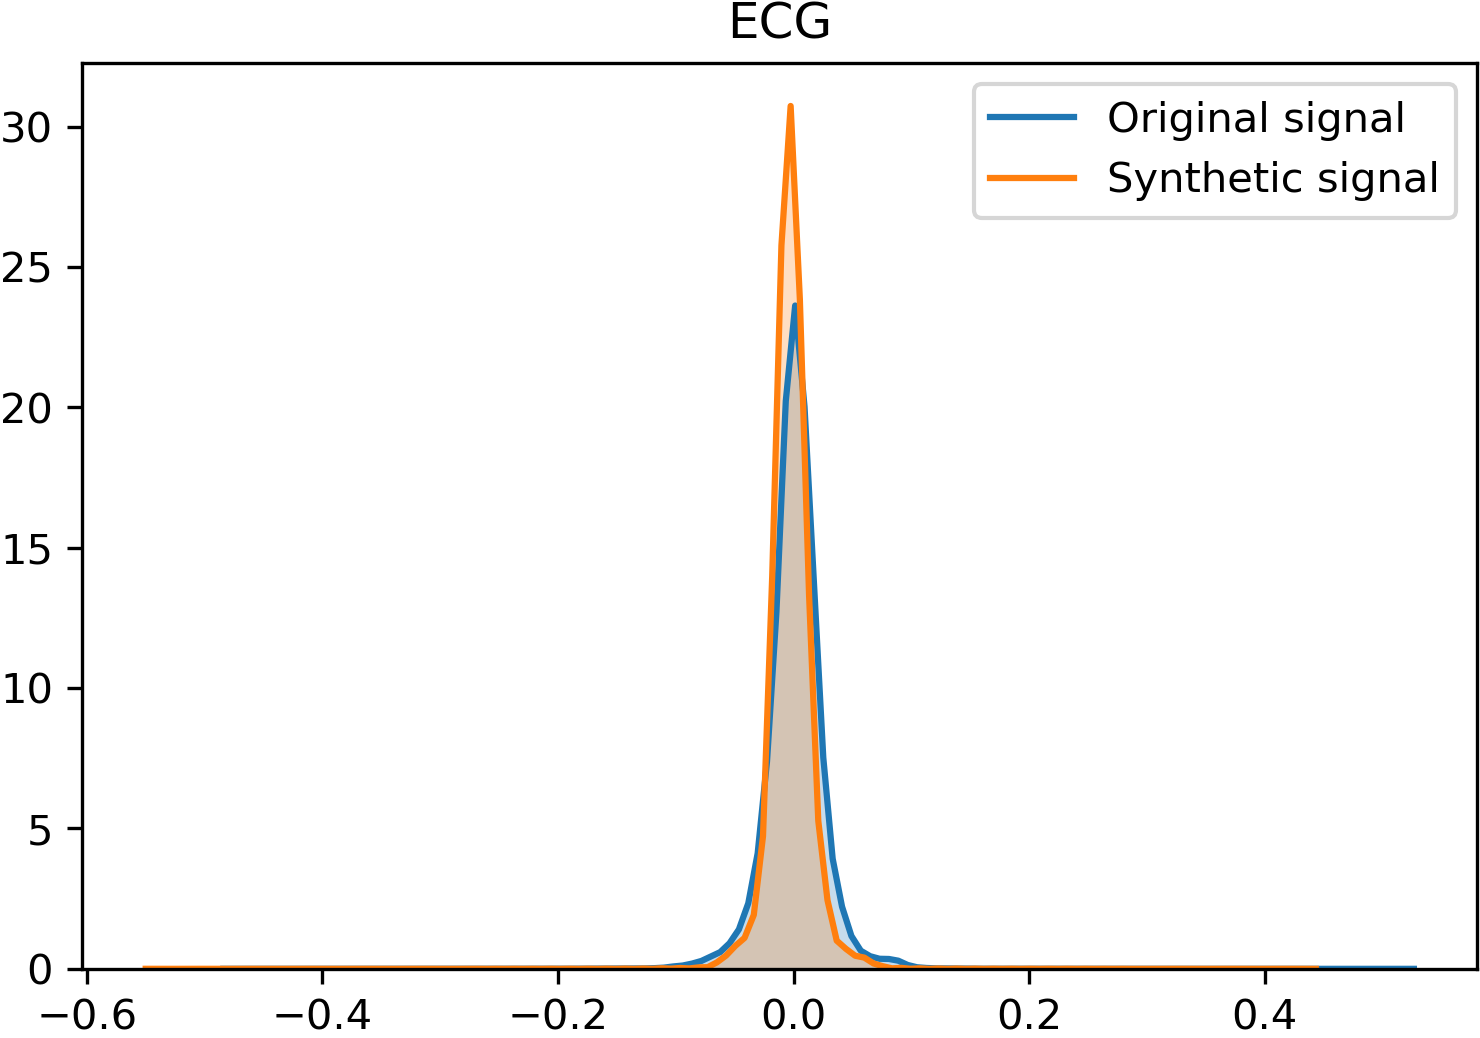
\includegraphics[width=.24\textwidth, height=2.8cm]{figs/dist_stress_ECG_acii2019_pres.png}\par
  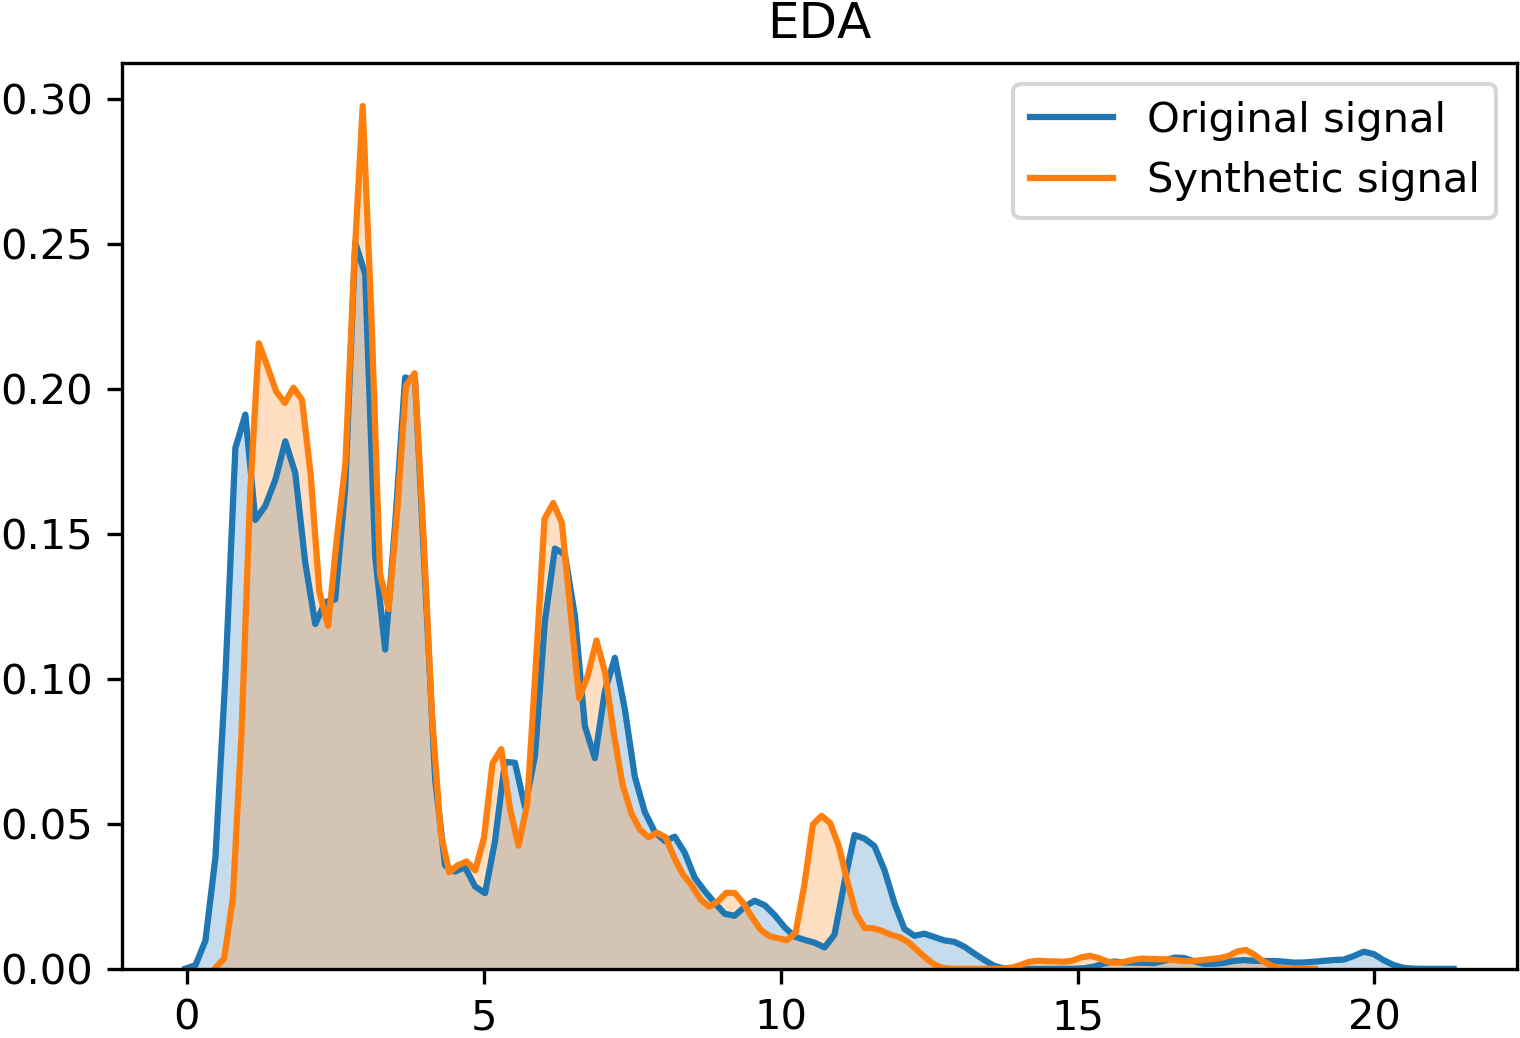
\includegraphics[width=.5\textwidth, height=5cm]{figs/dist_stress_EDA_acii2019_pres.png}\hfill
%   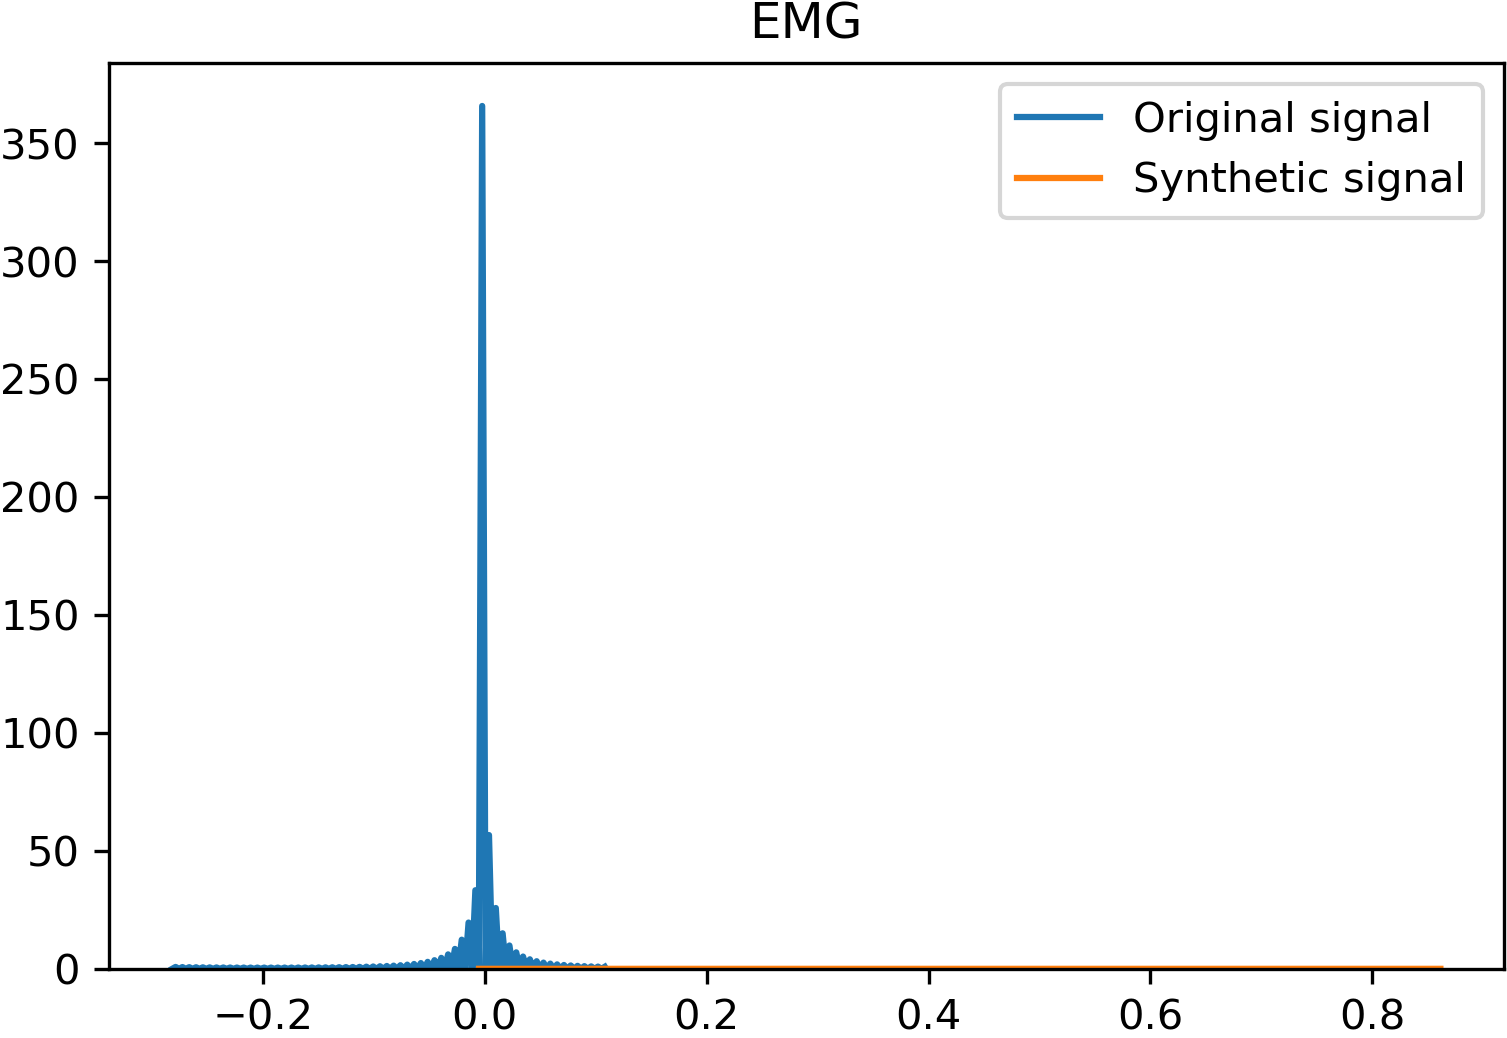
\includegraphics[width=.24\textwidth, height=2.8cm]{figs/dist_stress_EMG_acii2019_pres.png}\hfill
%   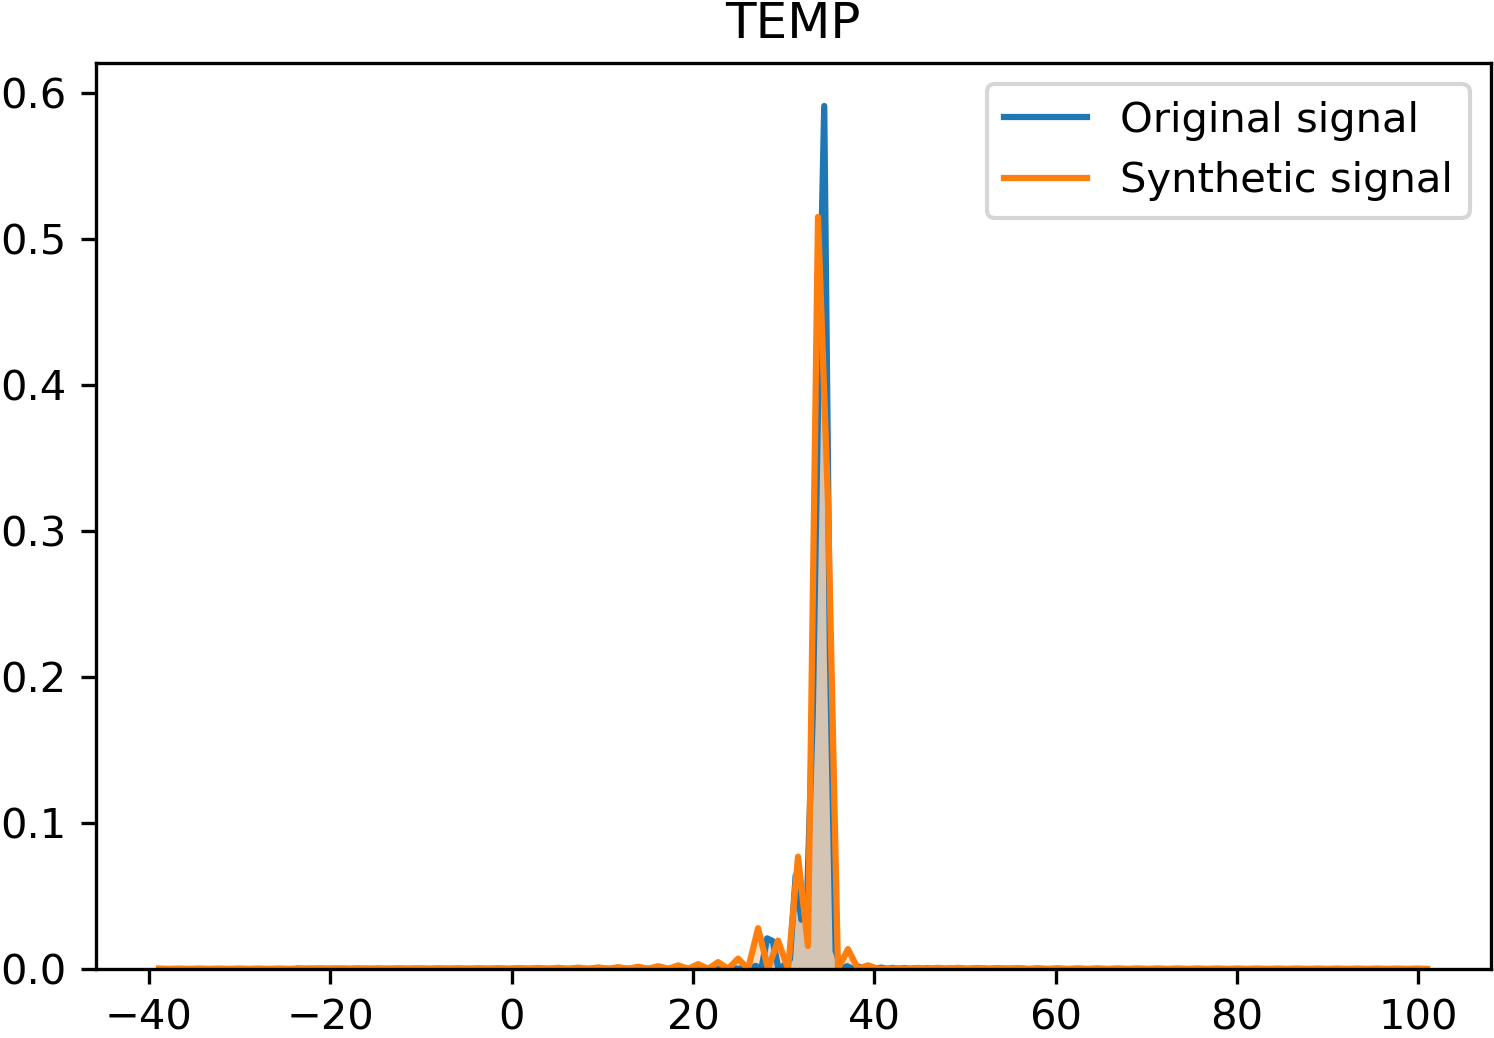
\includegraphics[width=.24\textwidth, height=2.8cm]{figs/dist_stress_Temp_acii2019_pres.png}\hfill
%   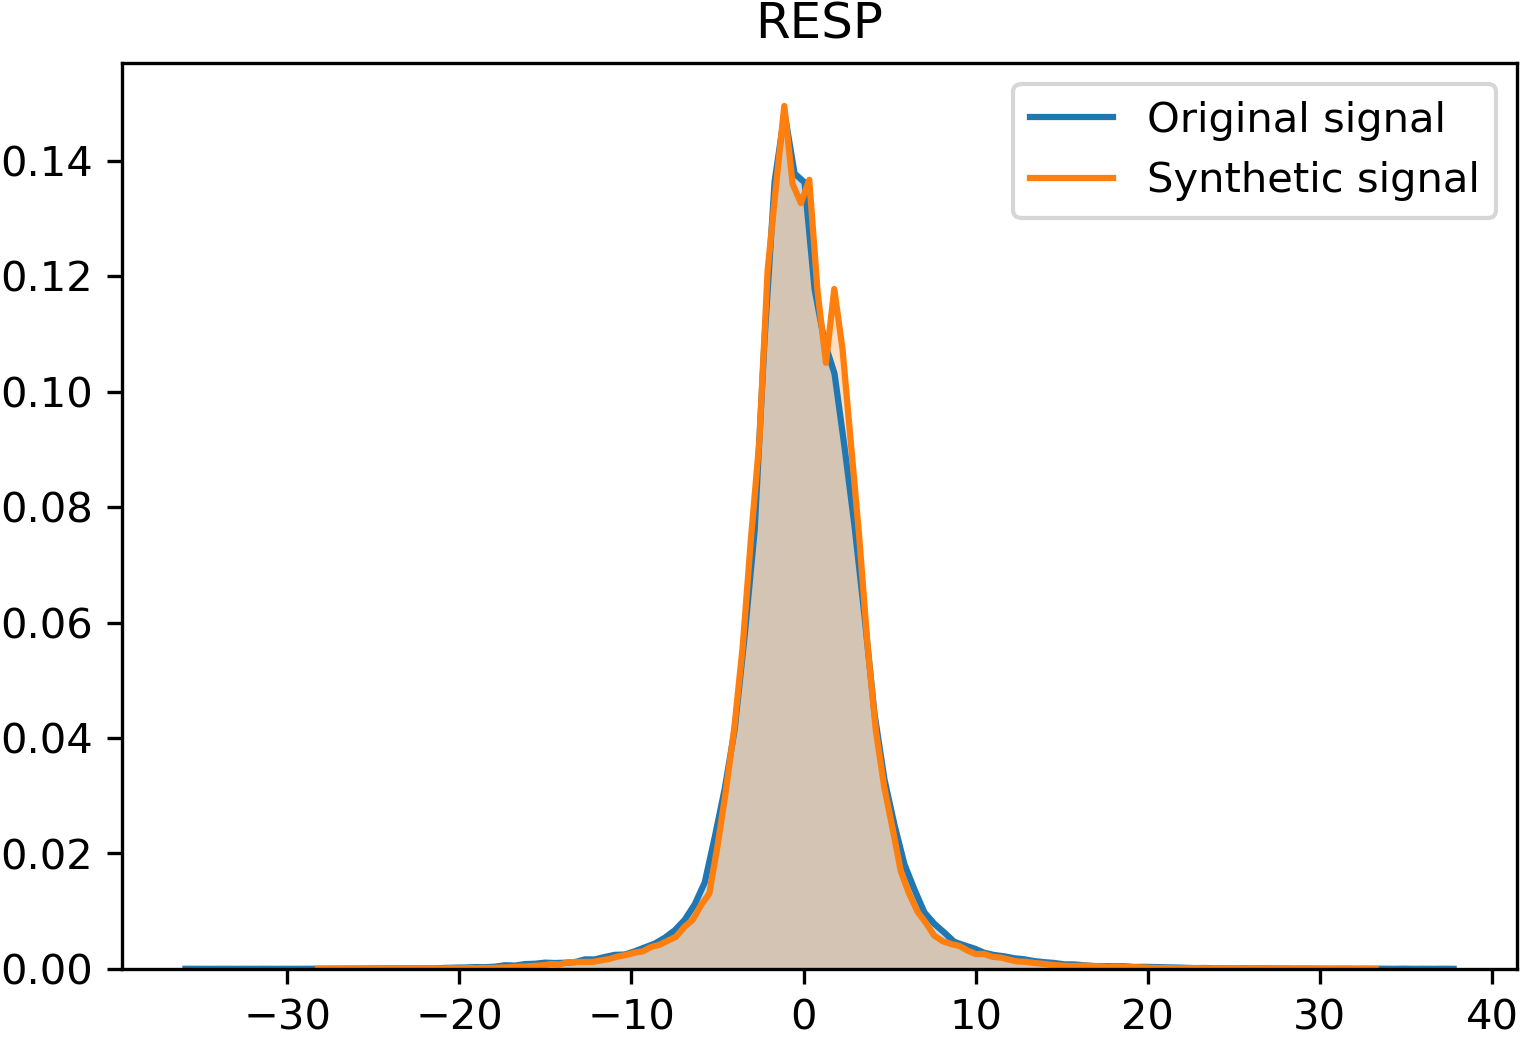
\includegraphics[width=.24\textwidth, height=2.8cm]{figs/dist_stress_Resp_acii2019_pres.png}\hfill

  \label{dist_plt}
\end{figure}

\end{frame}


\begin{frame}
\frametitle{Signal Distribution (Original and Synthesis)}

Learned the distribution for all signals except EMG

\begin{figure}
  \centering
  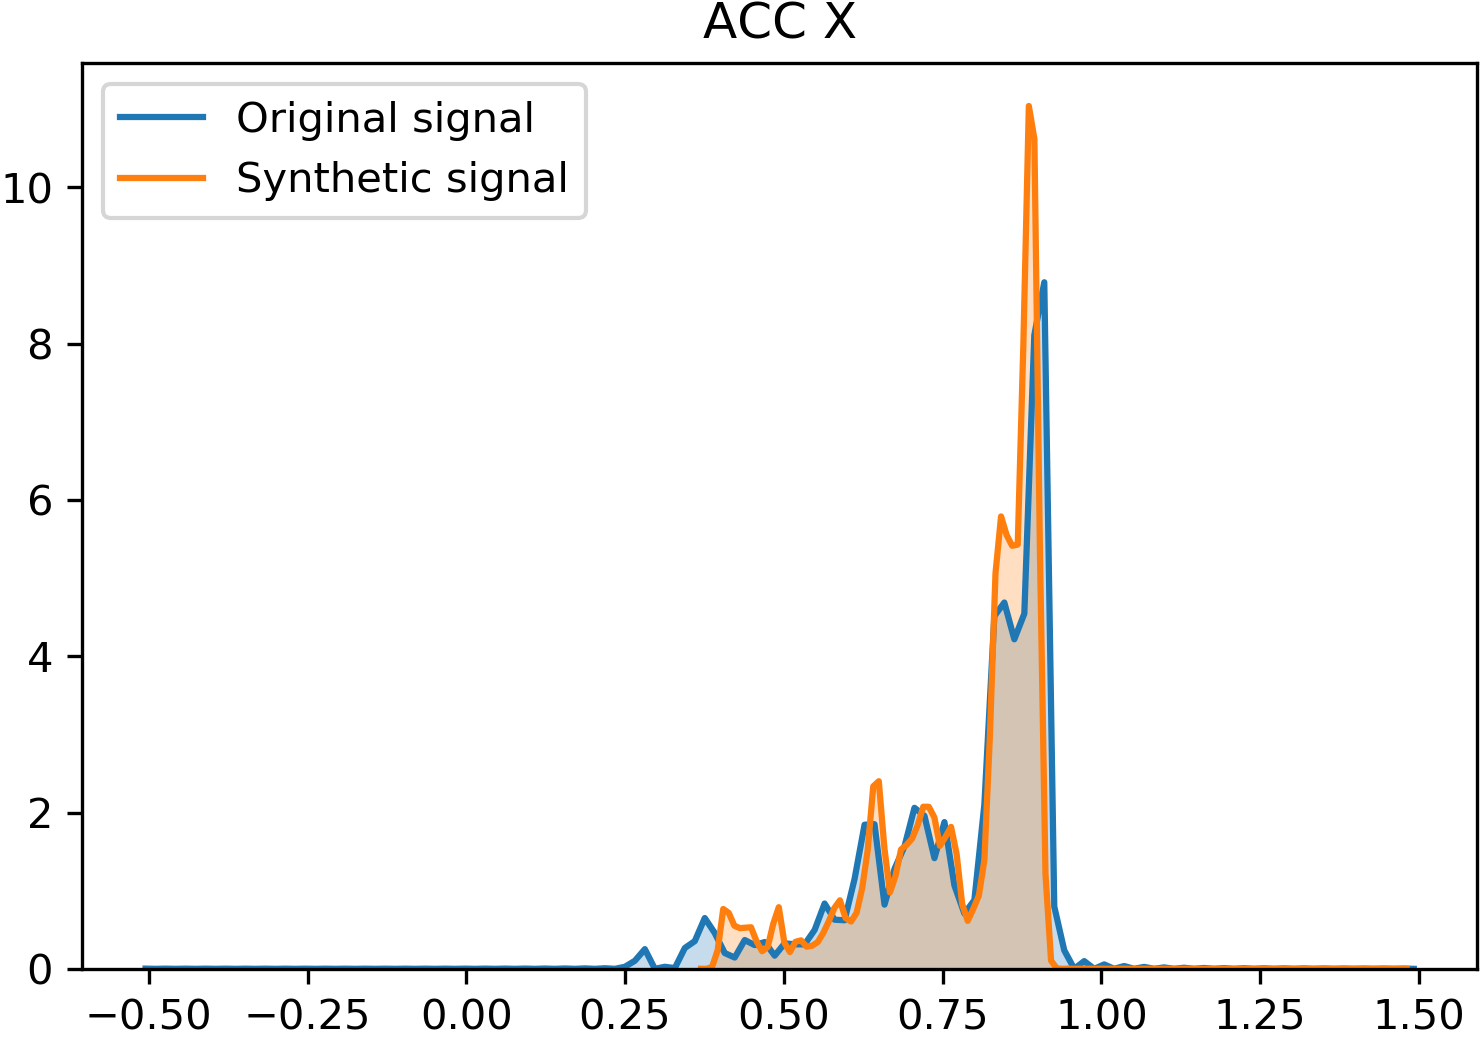
\includegraphics[width=.24\textwidth, height=2.8cm]{figs/dist_stress_ACC_X_acii2019_pres.png}\hfill
  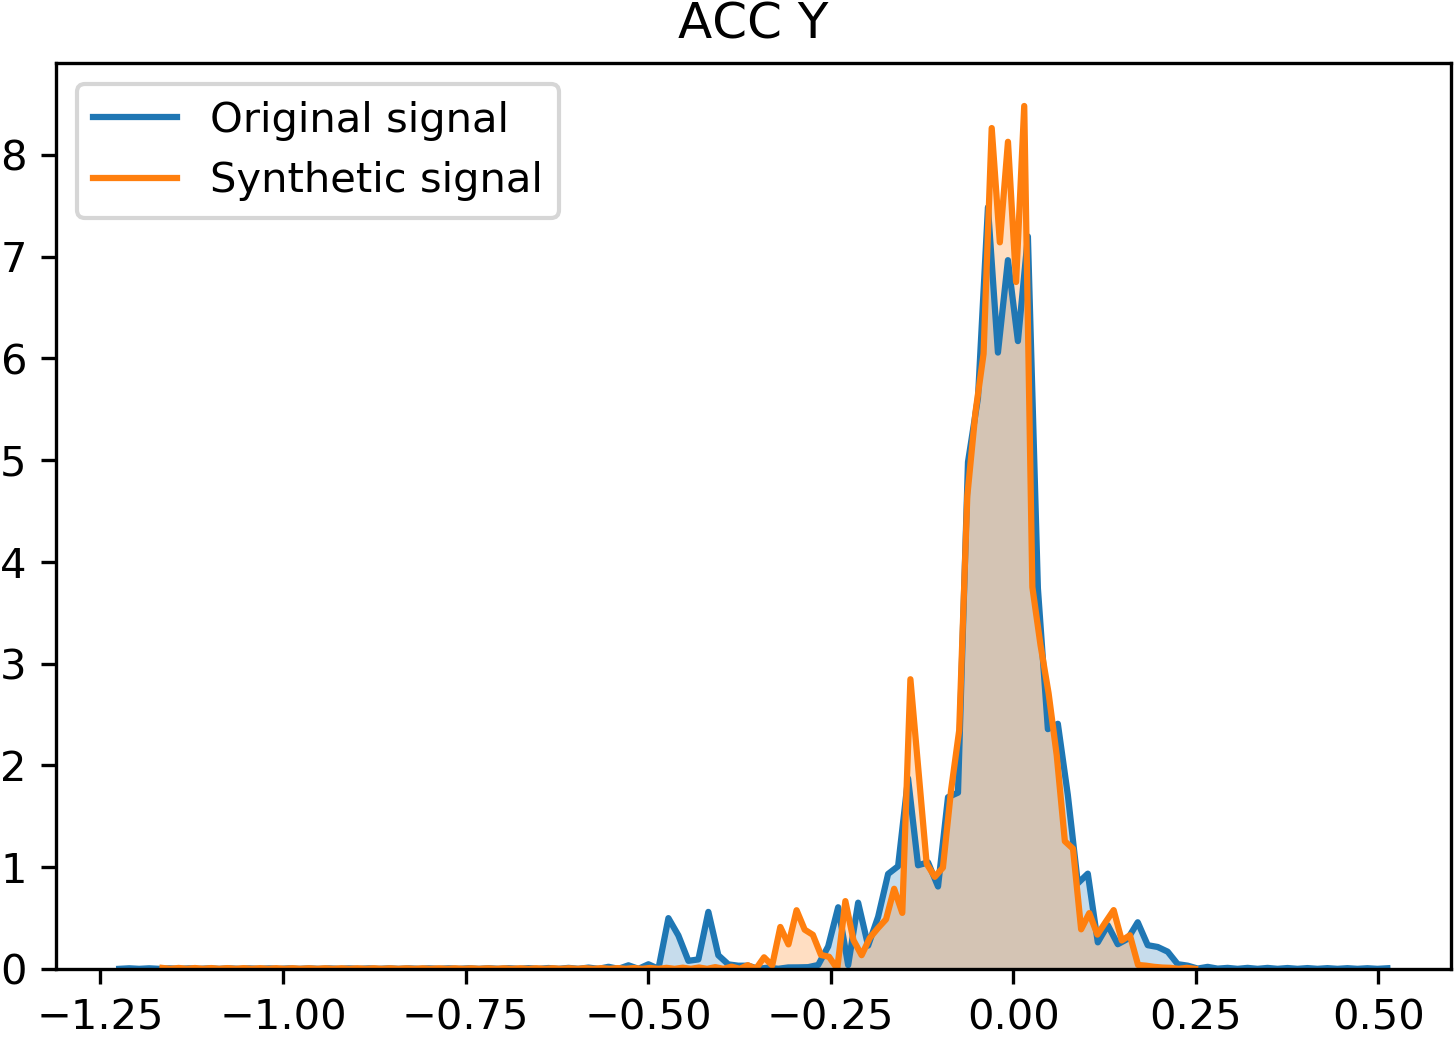
\includegraphics[width=.24\textwidth, height=2.8cm]{figs/dist_stress_ACC_Y_acii2019_pres.png}\hfill
  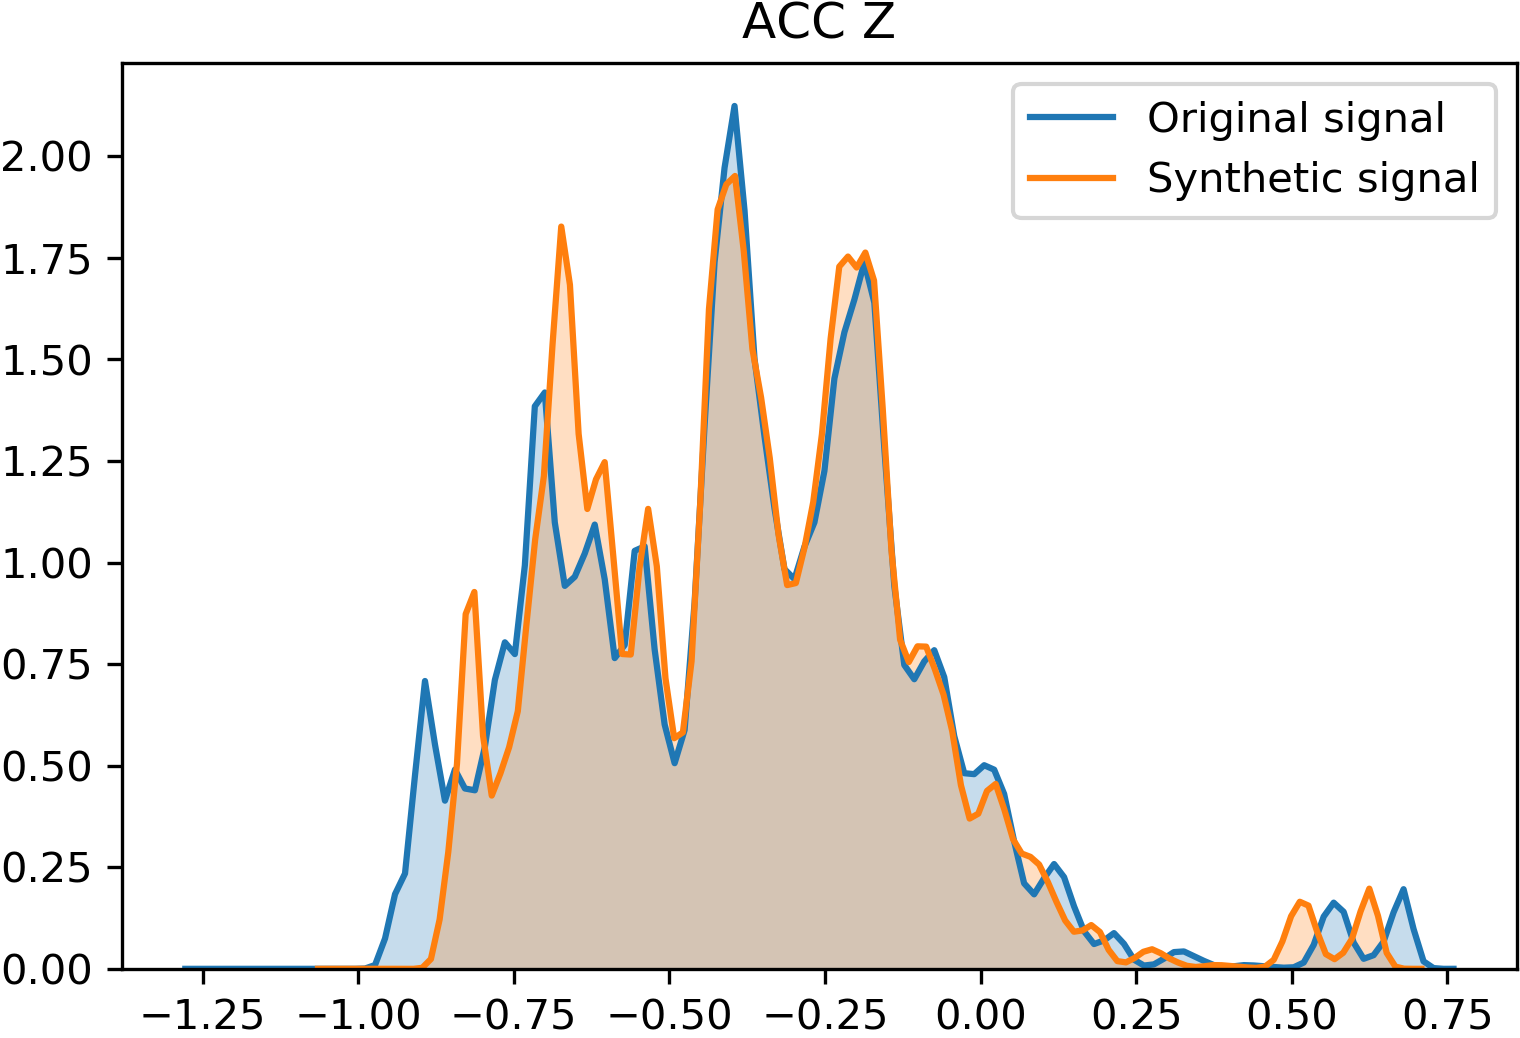
\includegraphics[width=.24\textwidth, height=2.8cm]{figs/dist_stress_ACC_Z_acii2019_pres.png}\hfill
  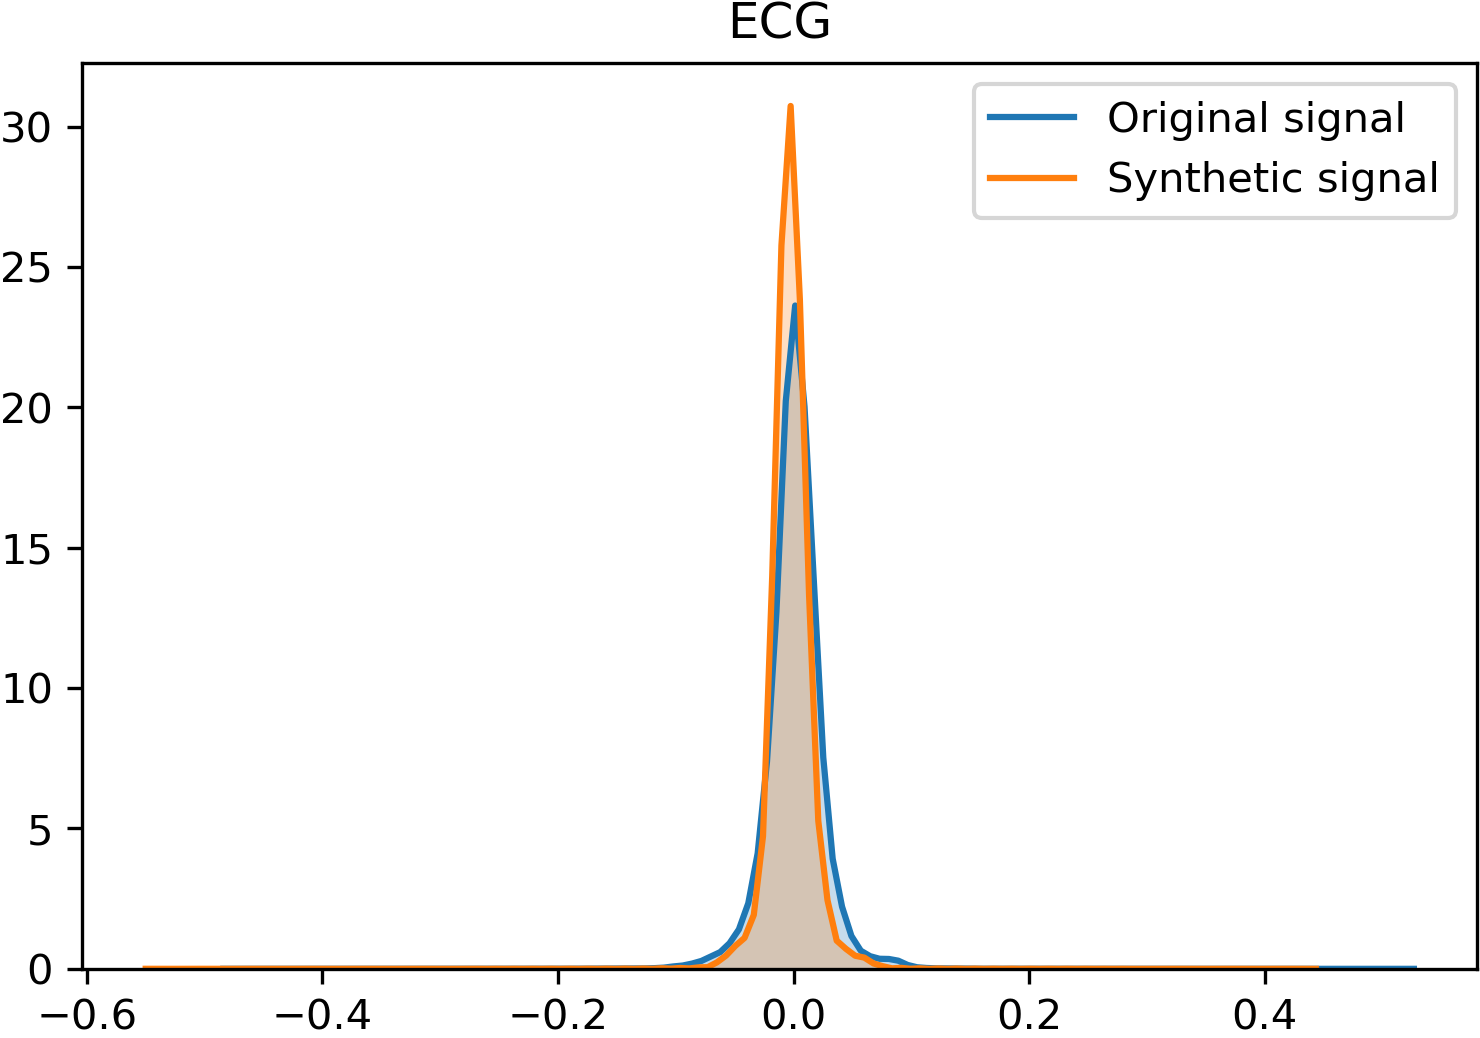
\includegraphics[width=.24\textwidth, height=2.8cm]{figs/dist_stress_ECG_acii2019_pres.png}\par
  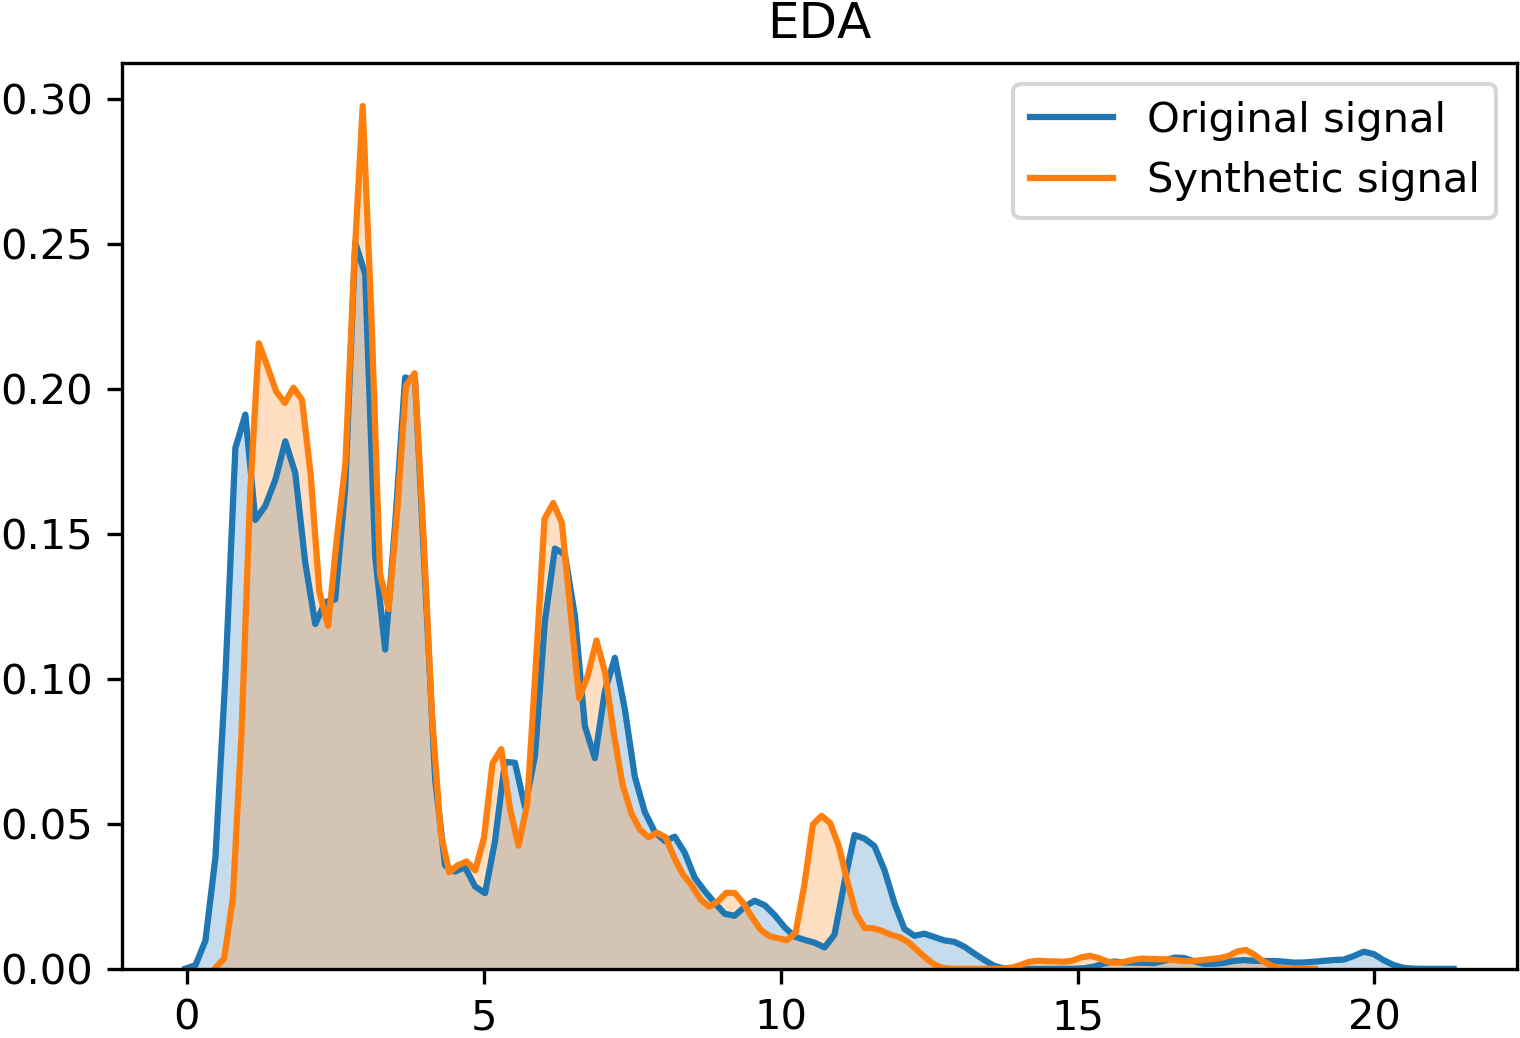
\includegraphics[width=.24\textwidth, height=2.8cm]{figs/dist_stress_EDA_acii2019_pres.png}\hfill
  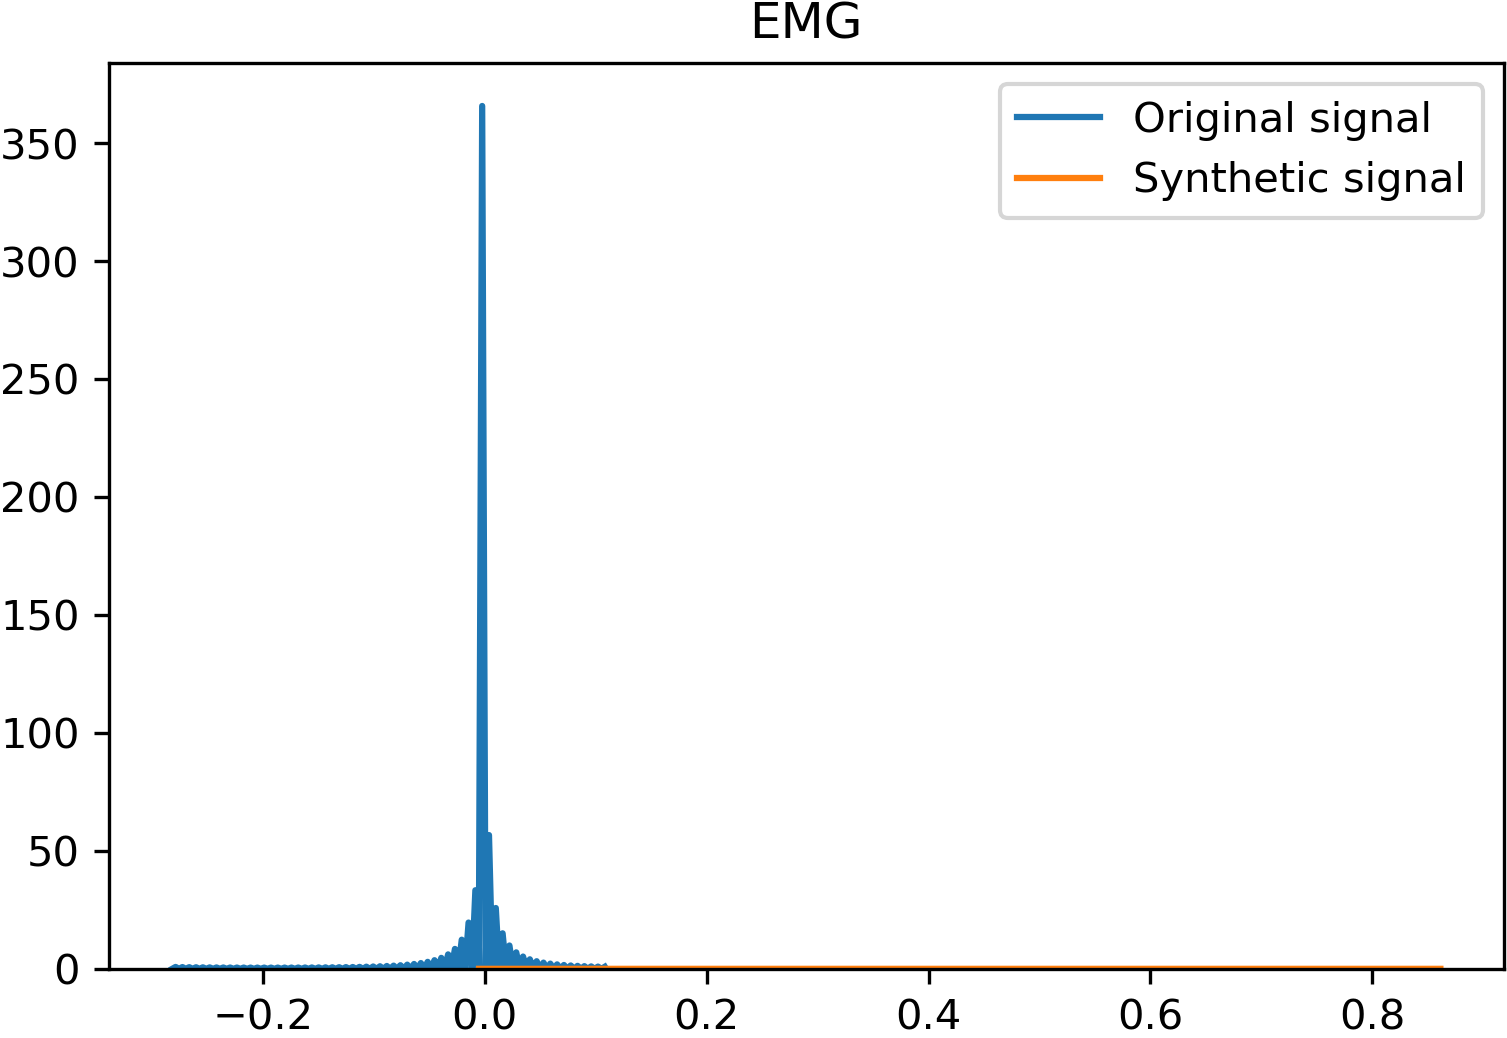
\includegraphics[width=.24\textwidth, height=2.8cm]{figs/dist_stress_EMG_acii2019_pres.png}\hfill
  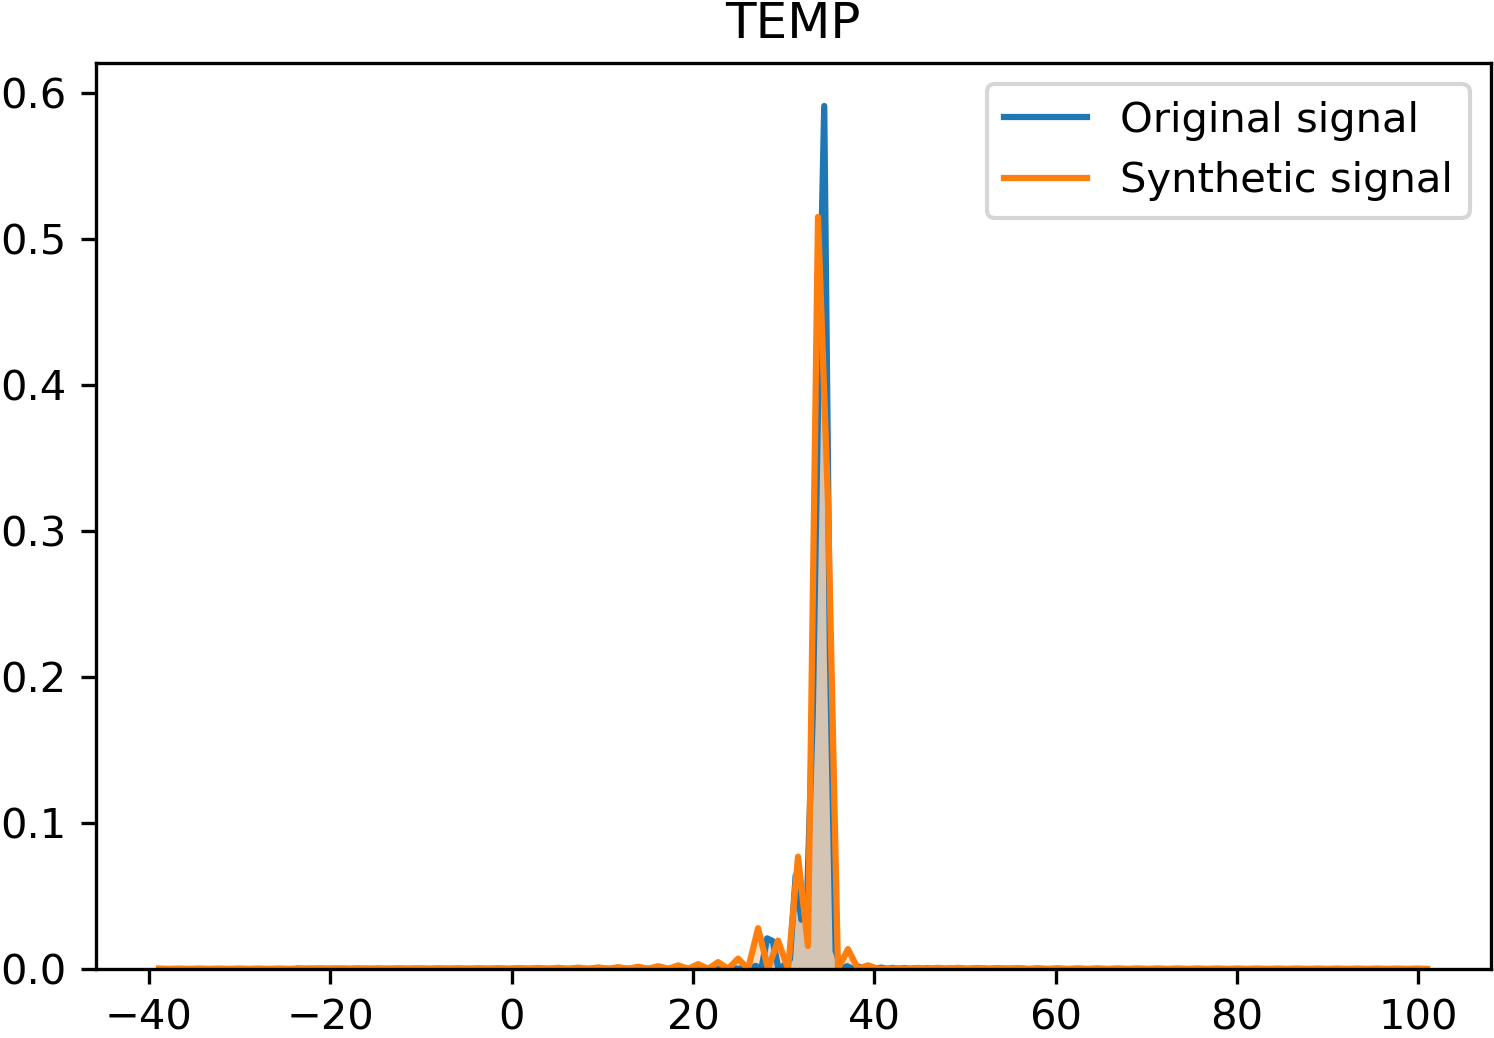
\includegraphics[width=.24\textwidth, height=2.8cm]{figs/dist_stress_Temp_acii2019_pres.png}\hfill
  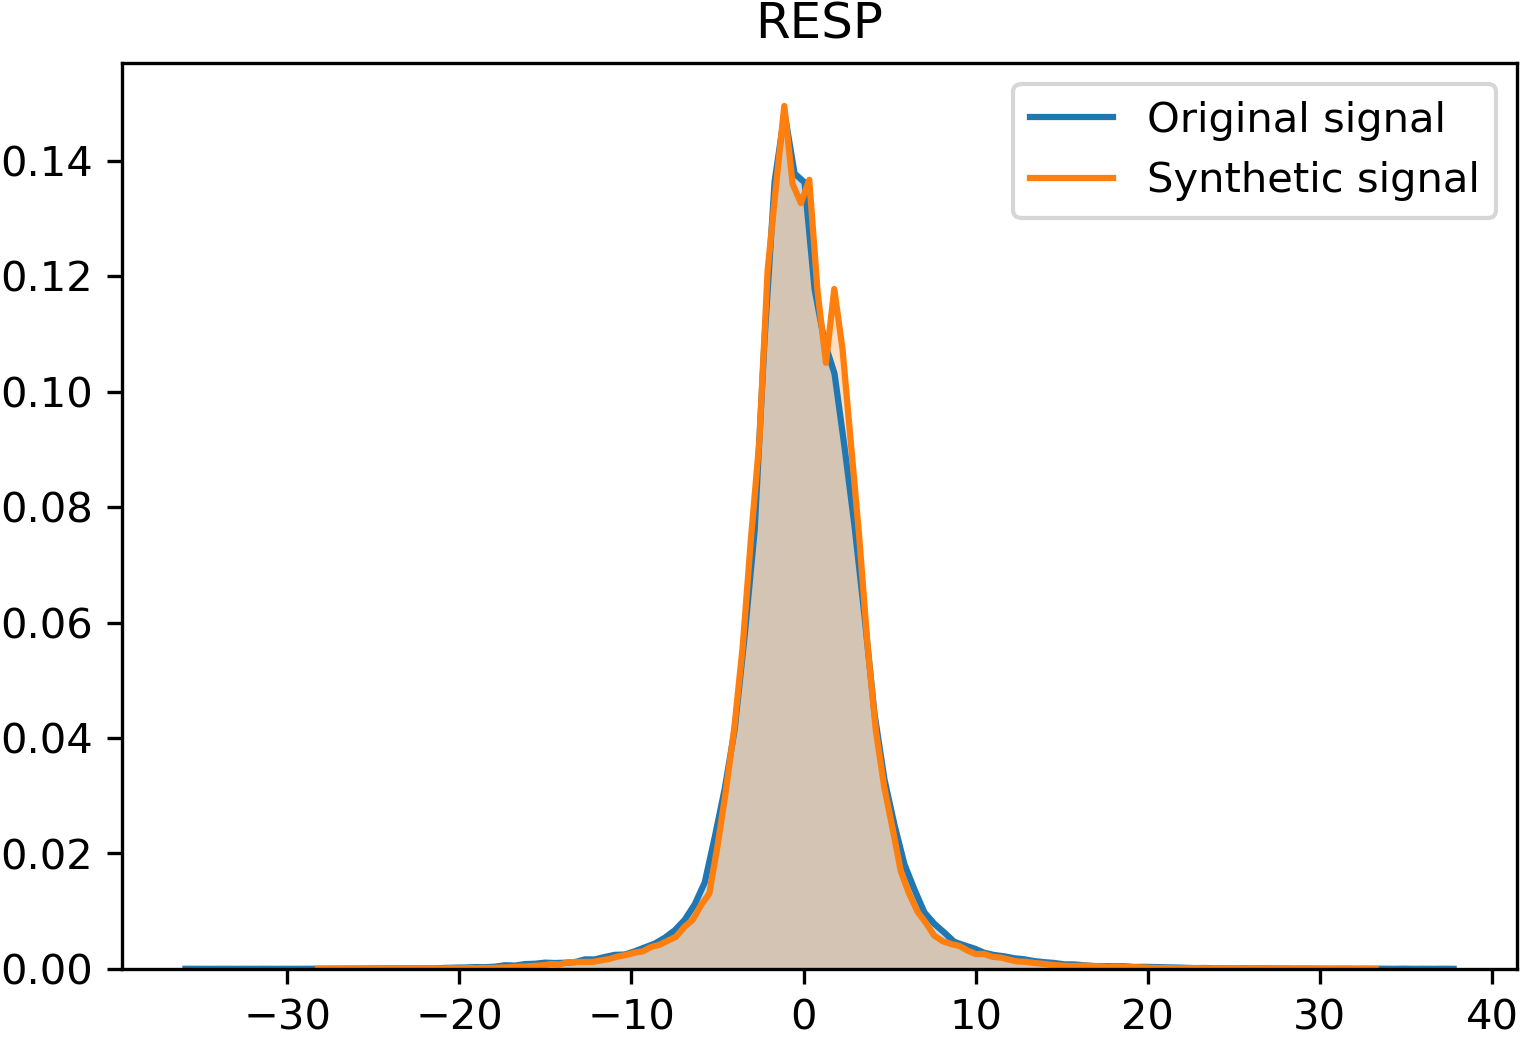
\includegraphics[width=.24\textwidth, height=2.8cm]{figs/dist_stress_Resp_acii2019_pres.png}\hfill

  \label{dist_plt}
\end{figure}

\end{frame}



\begin{frame}
\frametitle{Performance: Affect Prediction vs. Classification}

% Task: class stress from rest (baseline, amusement, meditation)

\begin{table}
    \tiny
    % \small
	\renewcommand{\arraystretch}{1.3}
	\label{table:classOrigSynth}
	
	\label{cls_perf}
	\centering
	\begin{tabular}{lllllll}
	    \hline
	    \bfseries Detection Setting & & \bfseries Original data & &  & \bfseries Synthetic data & \\
		% \hline
		 & Precision  & Recall  & F1-score & Precision  & Recall  & F1-score \\
% 		\hline
		%\hline
        \hline
		Stress vs Baseline  &   0.71$\pm$0.06   &  0.68$\pm$0.10 &   0.69$\pm$0.08   & 0.71$\pm$0.10  & 0.66$\pm$0.11 & 0.68$\pm$0.10 \\
		\pause Stress vs Amusement  &   0.54$\pm$0.11   &  0.61$\pm$0.06 &   0.57$\pm$0.10   & 0.55$\pm$0.15  & 0.56$\pm$0.07 & 0.55$\pm$0.11 \\
		\pause Stress vs Meditation &   0.72$\pm$0.05   &  0.71$\pm$0.06 &   0.71$\pm$0.06   & 0.71$\pm$0.02  & 0.7$\pm$0.02 & 0.71$\pm$0.02 \\
		\pause Stress vs Rest &   0.76$\pm$0.03   &  0.7$\pm$0.06 &   0.73$\pm$0.04   & 0.74$\pm$0.03  & 0.67$\pm$0.07 & 0.7$\pm$0.04 \\
		\hline
	\end{tabular}
	% \caption{Classification results on both original and synthetic WESAD dataset using random forest.
	% }
\end{table}


\end{frame}

%------------------------------------------------
\section{Conclusion and Discussion}
%------------------------------------------------

\begin{frame}
\frametitle{Summary, Challenges and Future Work}

\begin{enumerate}[]
    \pause \item \textbf{Summary} \\
        \begin{enumerate}[-]
            \item Predicted signal ahead of time using CNN
            \item Detected affective states from predicted (synthetic) data 
            \item Achieved comparable results \newline 
        \end{enumerate}
        
    \pause \item \textbf{Challenges and Future Work} \\
    
    % TODO: Gender, Improve EMG, ECG
        \begin{enumerate}[-]
        \item Synthetic data to synthesize data. (Noise, drift) $\longrightarrow$ out of distribuution (Alcorn et al., CVPR 2019)
        \item Influence of gender (male \& female) 
        \item Explore EMG and ECG
        \end{enumerate}
\end{enumerate}

\end{frame}


%\begin{frame}
%\frametitle{  }

%\center Thank you! \newline 

% \center QAs


%\end{frame}


\end{document}